\chapter{Appendix}

\section{First set of molecules (set-up failed)}

\begin{figure}[h!]
	
	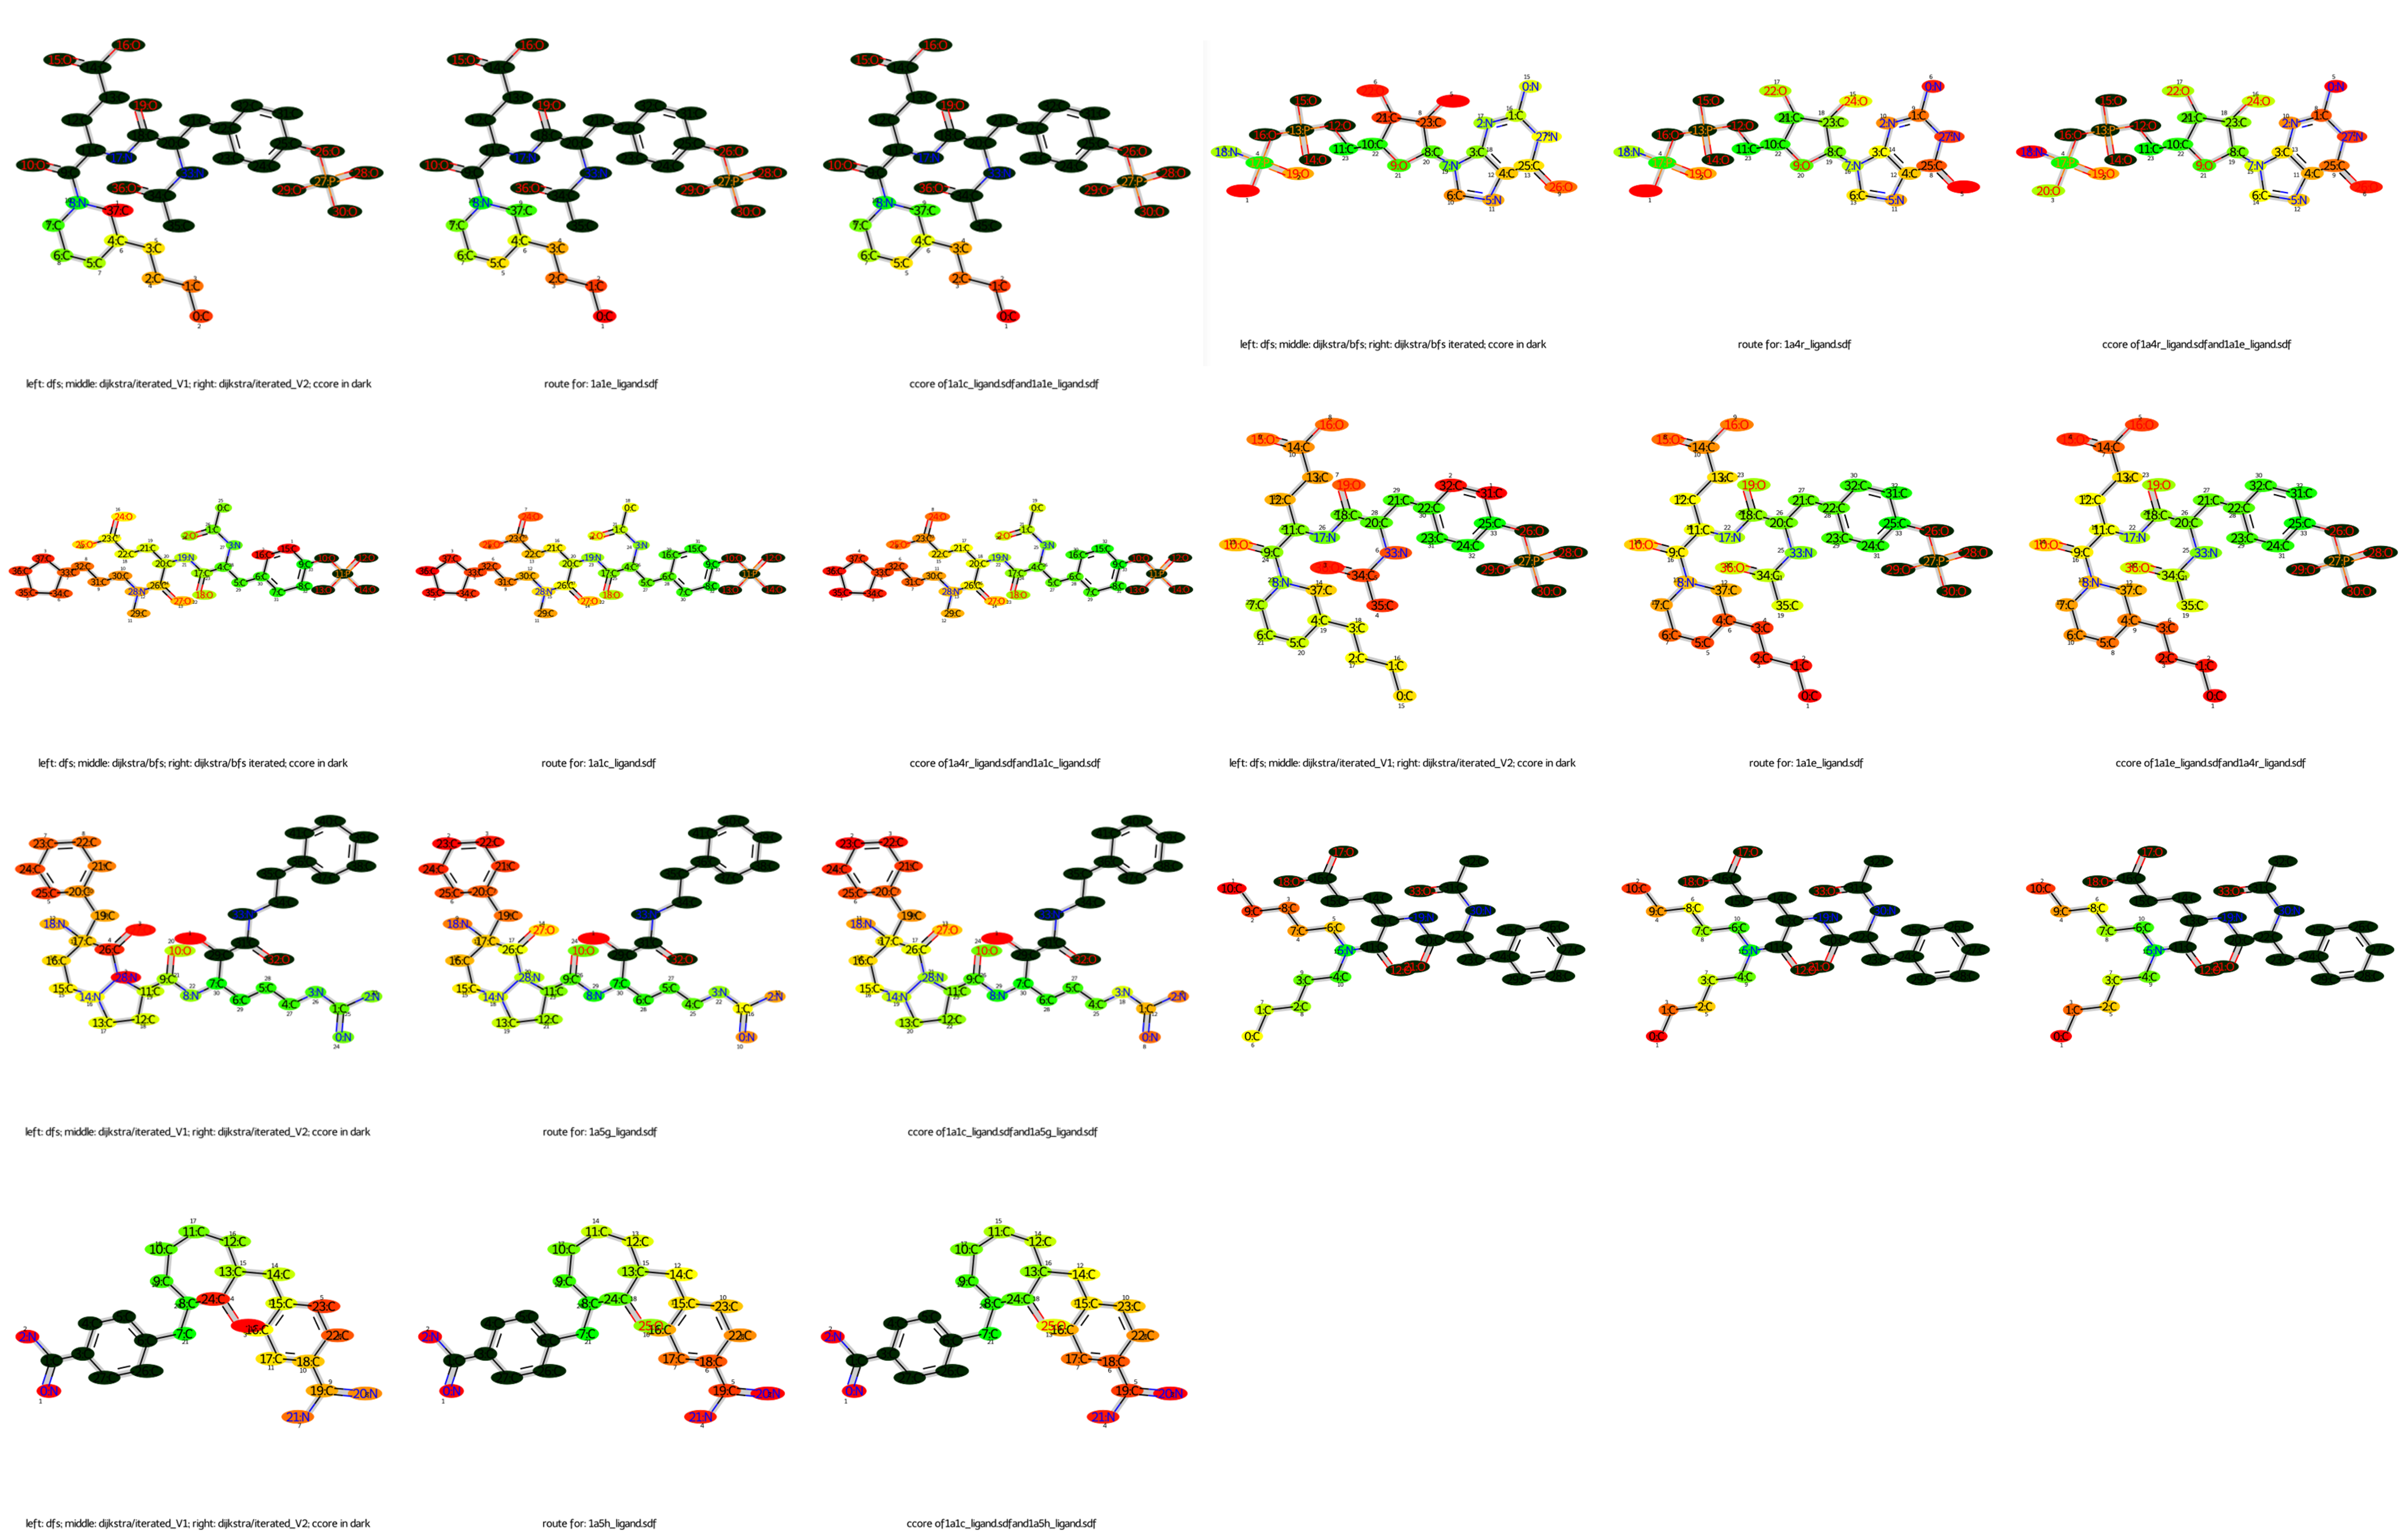
\includegraphics[scale=0.50]{routes_first_set_failed}\caption{left: DFS-algorithm; middle: BFS-iter-algorithm; right: BFS-iter+-algorithm; common core in dark}
	
\end{figure}

\section{Second set of molecules}

\begin{figure}[H]
	
	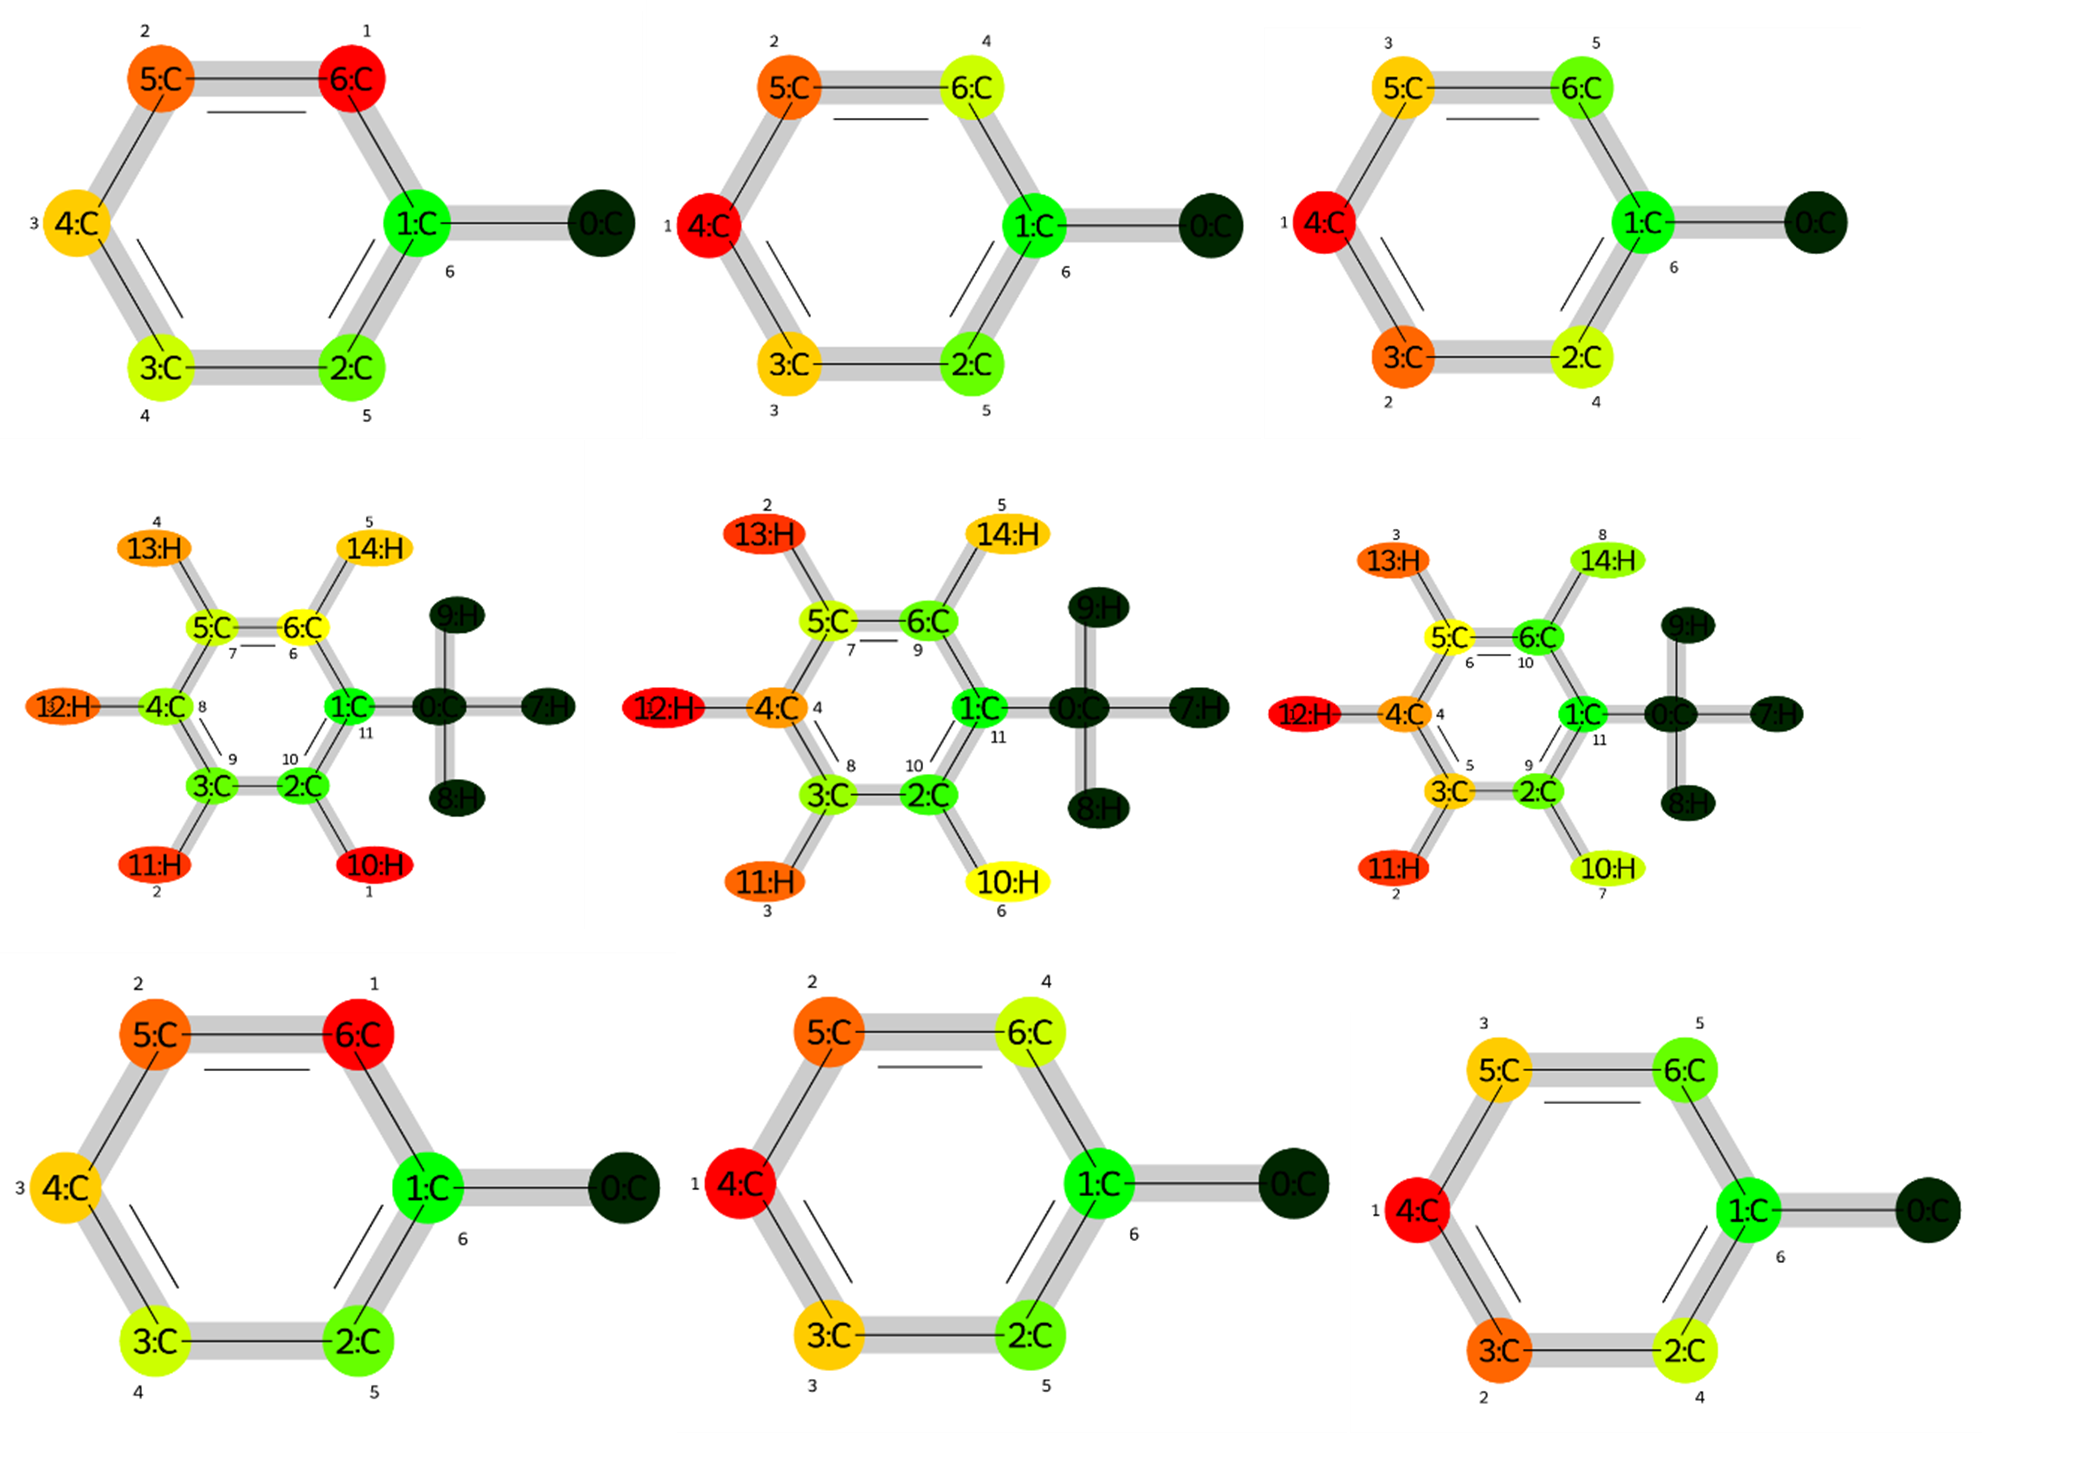
\includegraphics[scale=0.75]{toluene_set2}\caption{Toluene->Methanol; first row: correct common core and mutation route, hydrogens excluded; middle row: hydrogens included; right: hydrogens included, but removed before drawing; left: DFS-algorithm; middle: BFS-algorithm; right: BFS-iter-algorithm; common core in dark, for these small molecules the differences between the new mutation algorithms (i.e. middle and right) are negligible}
	
\end{figure}


\begin{figure}[H]
	
	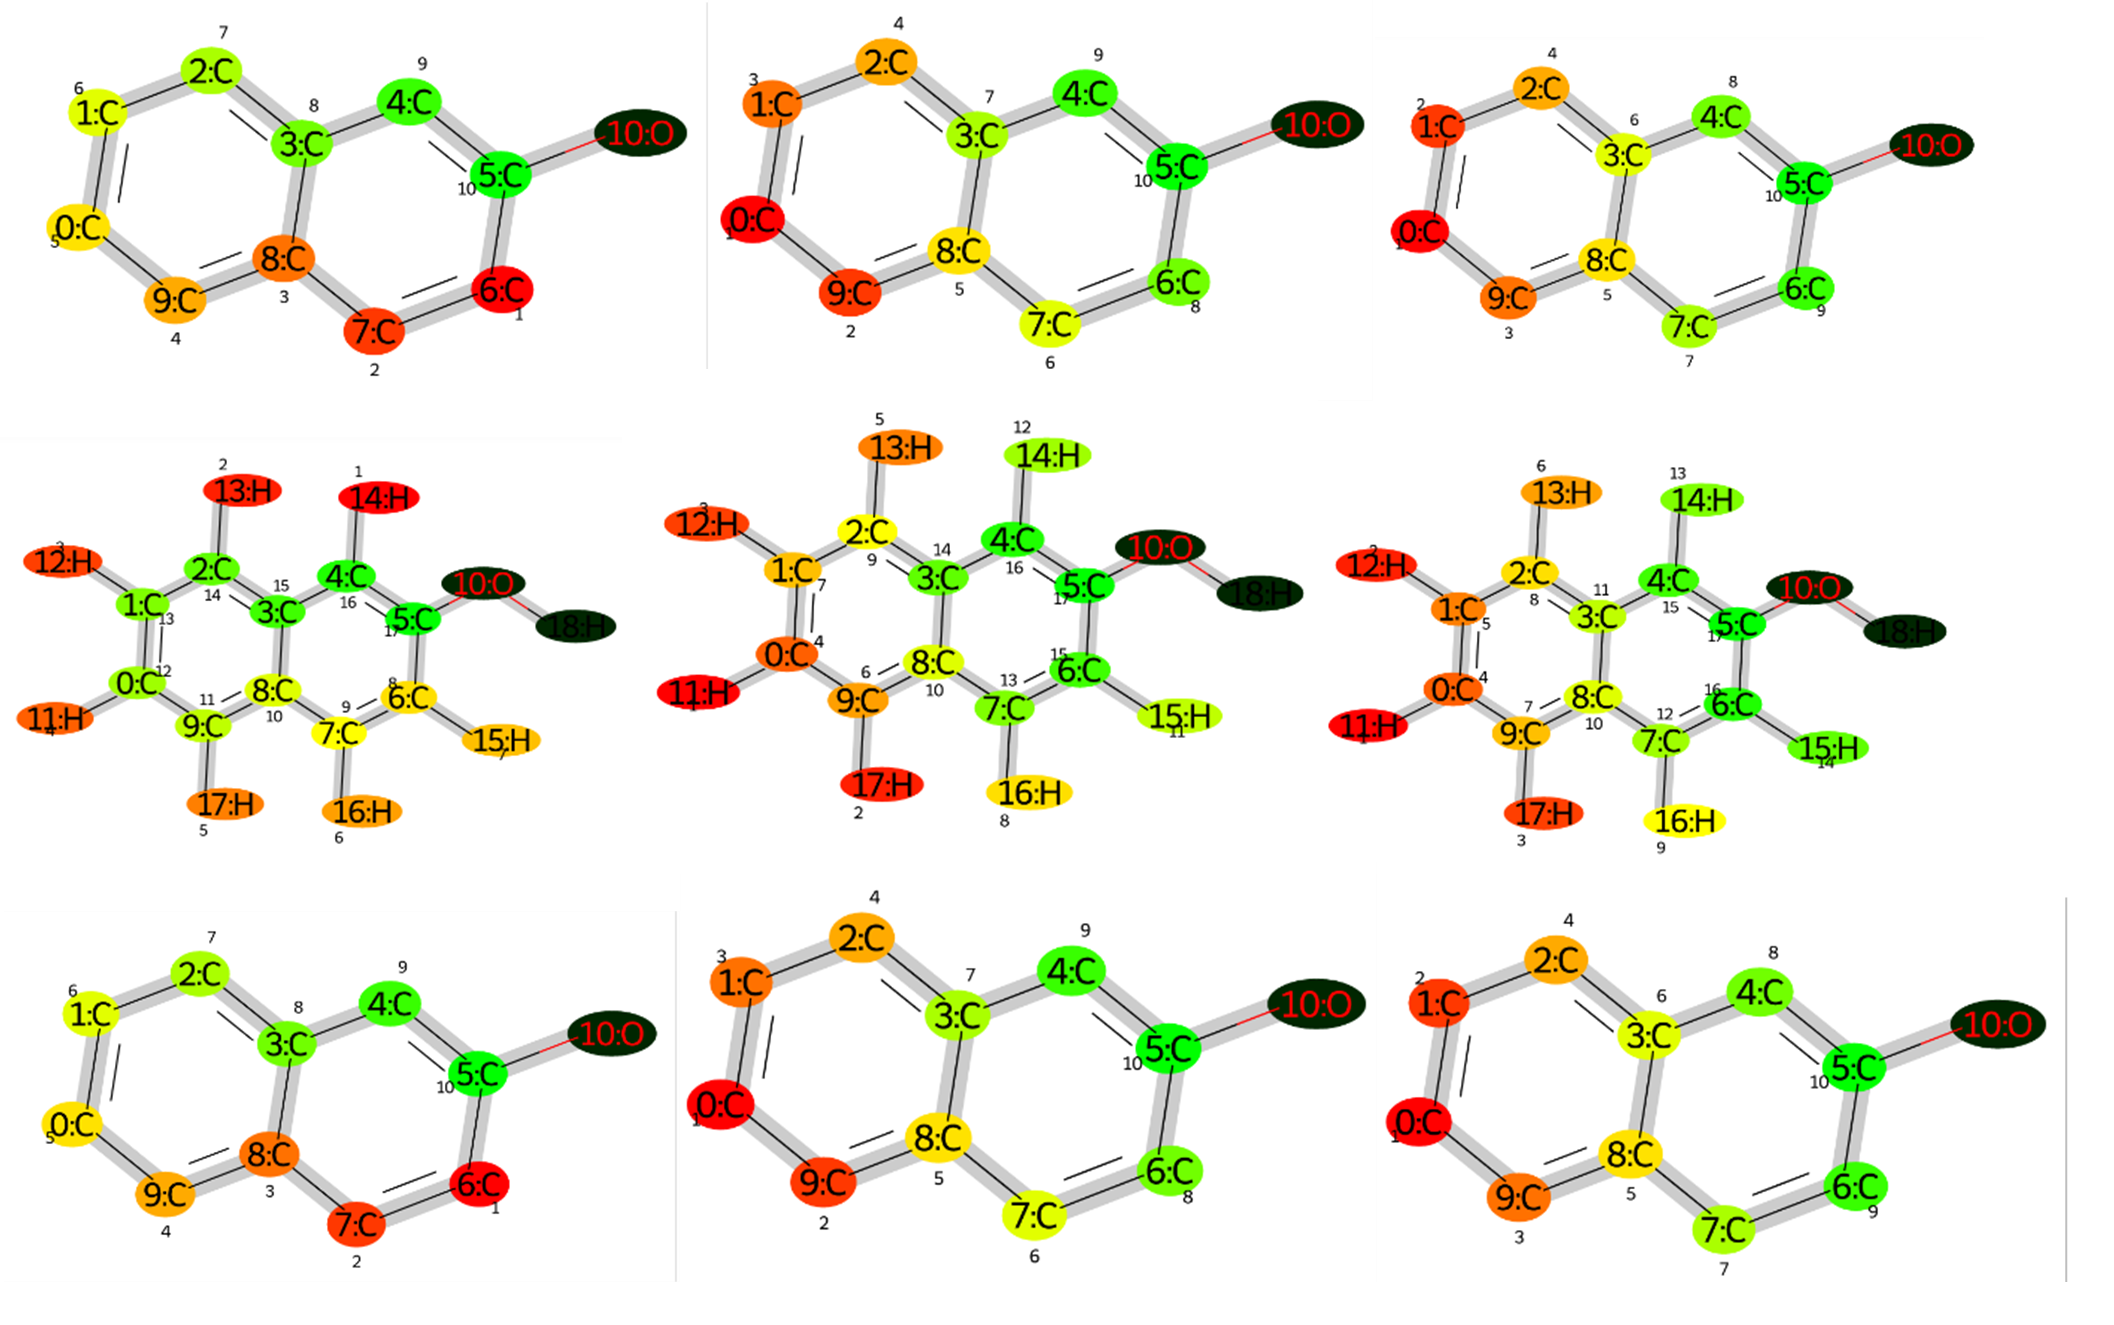
\includegraphics[scale=0.75]{2naphthol_set2}\caption{mutation route for 2-naphthol for 2-naphthol->methanol; first row: correct common core and mutation route, hydrogens excluded; middle row: hydrogens included; right: hydrogens included, but removed before drawing; left: DFS-algorithm; middle: BFS-algorithm; right: BFS-iter-algorithm; common core in dark, for these small molecules the differences between the new mutation algorithms (i.e. middle and right) are negligible}
	
\end{figure}

\begin{figure}[H]
	
	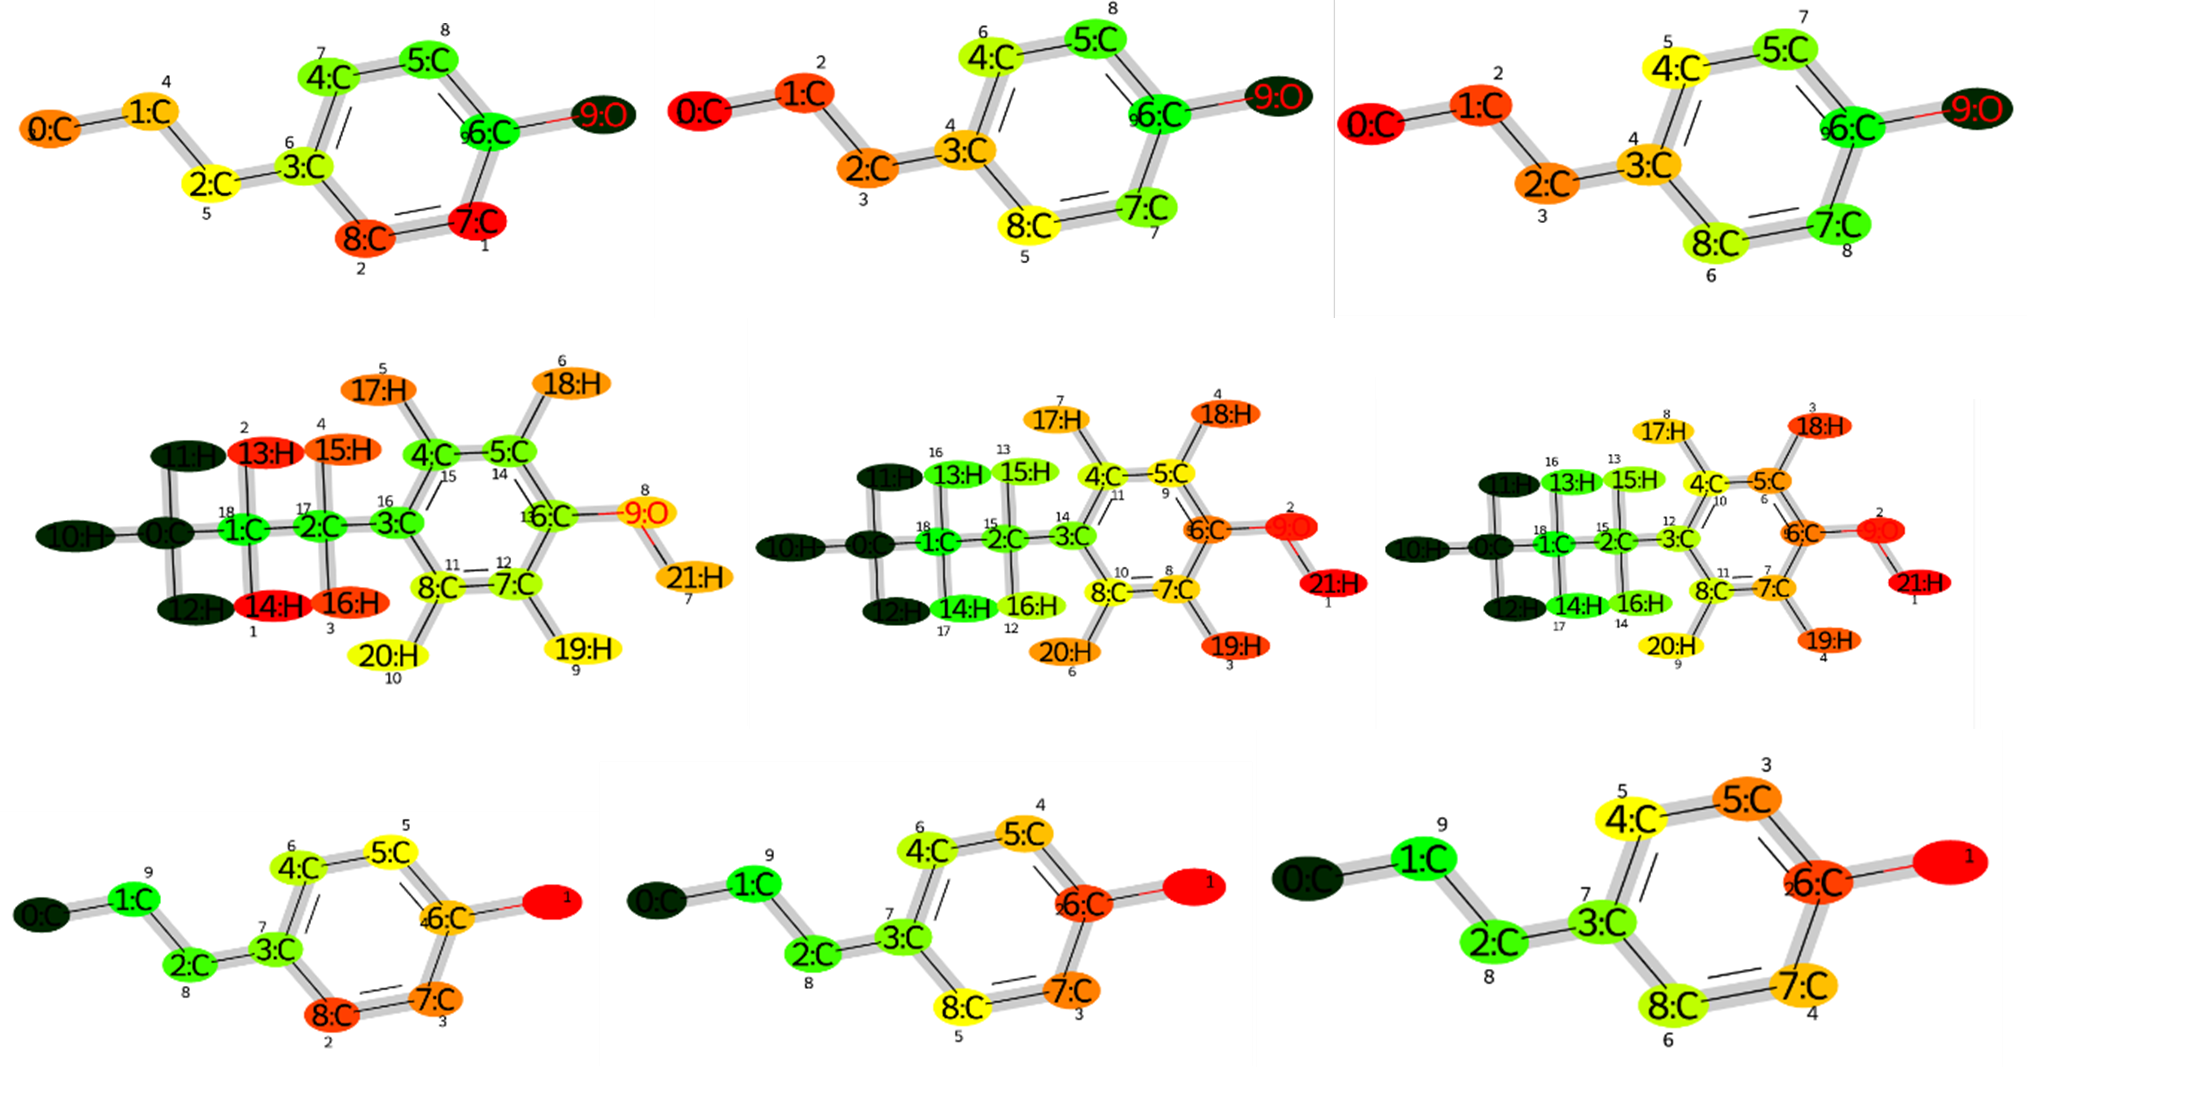
\includegraphics[scale=0.75]{6propylphenol_set2}\caption{mutation route for 6-propylphenol for 6-propylphenol->methanol; first row: correct common core and mutation route, hydrogens excluded; middle row: hydrogens included; right: hydrogens included, but removed before drawing; left: DFS-algorithm; middle: BFS-algorithm; right: BFS-iter-algorithm; common core in dark, for these small molecules the differences between the new mutation algorithms (i.e. middle and right) are negligible}
	
\end{figure}

\begin{figure}[H]
	
	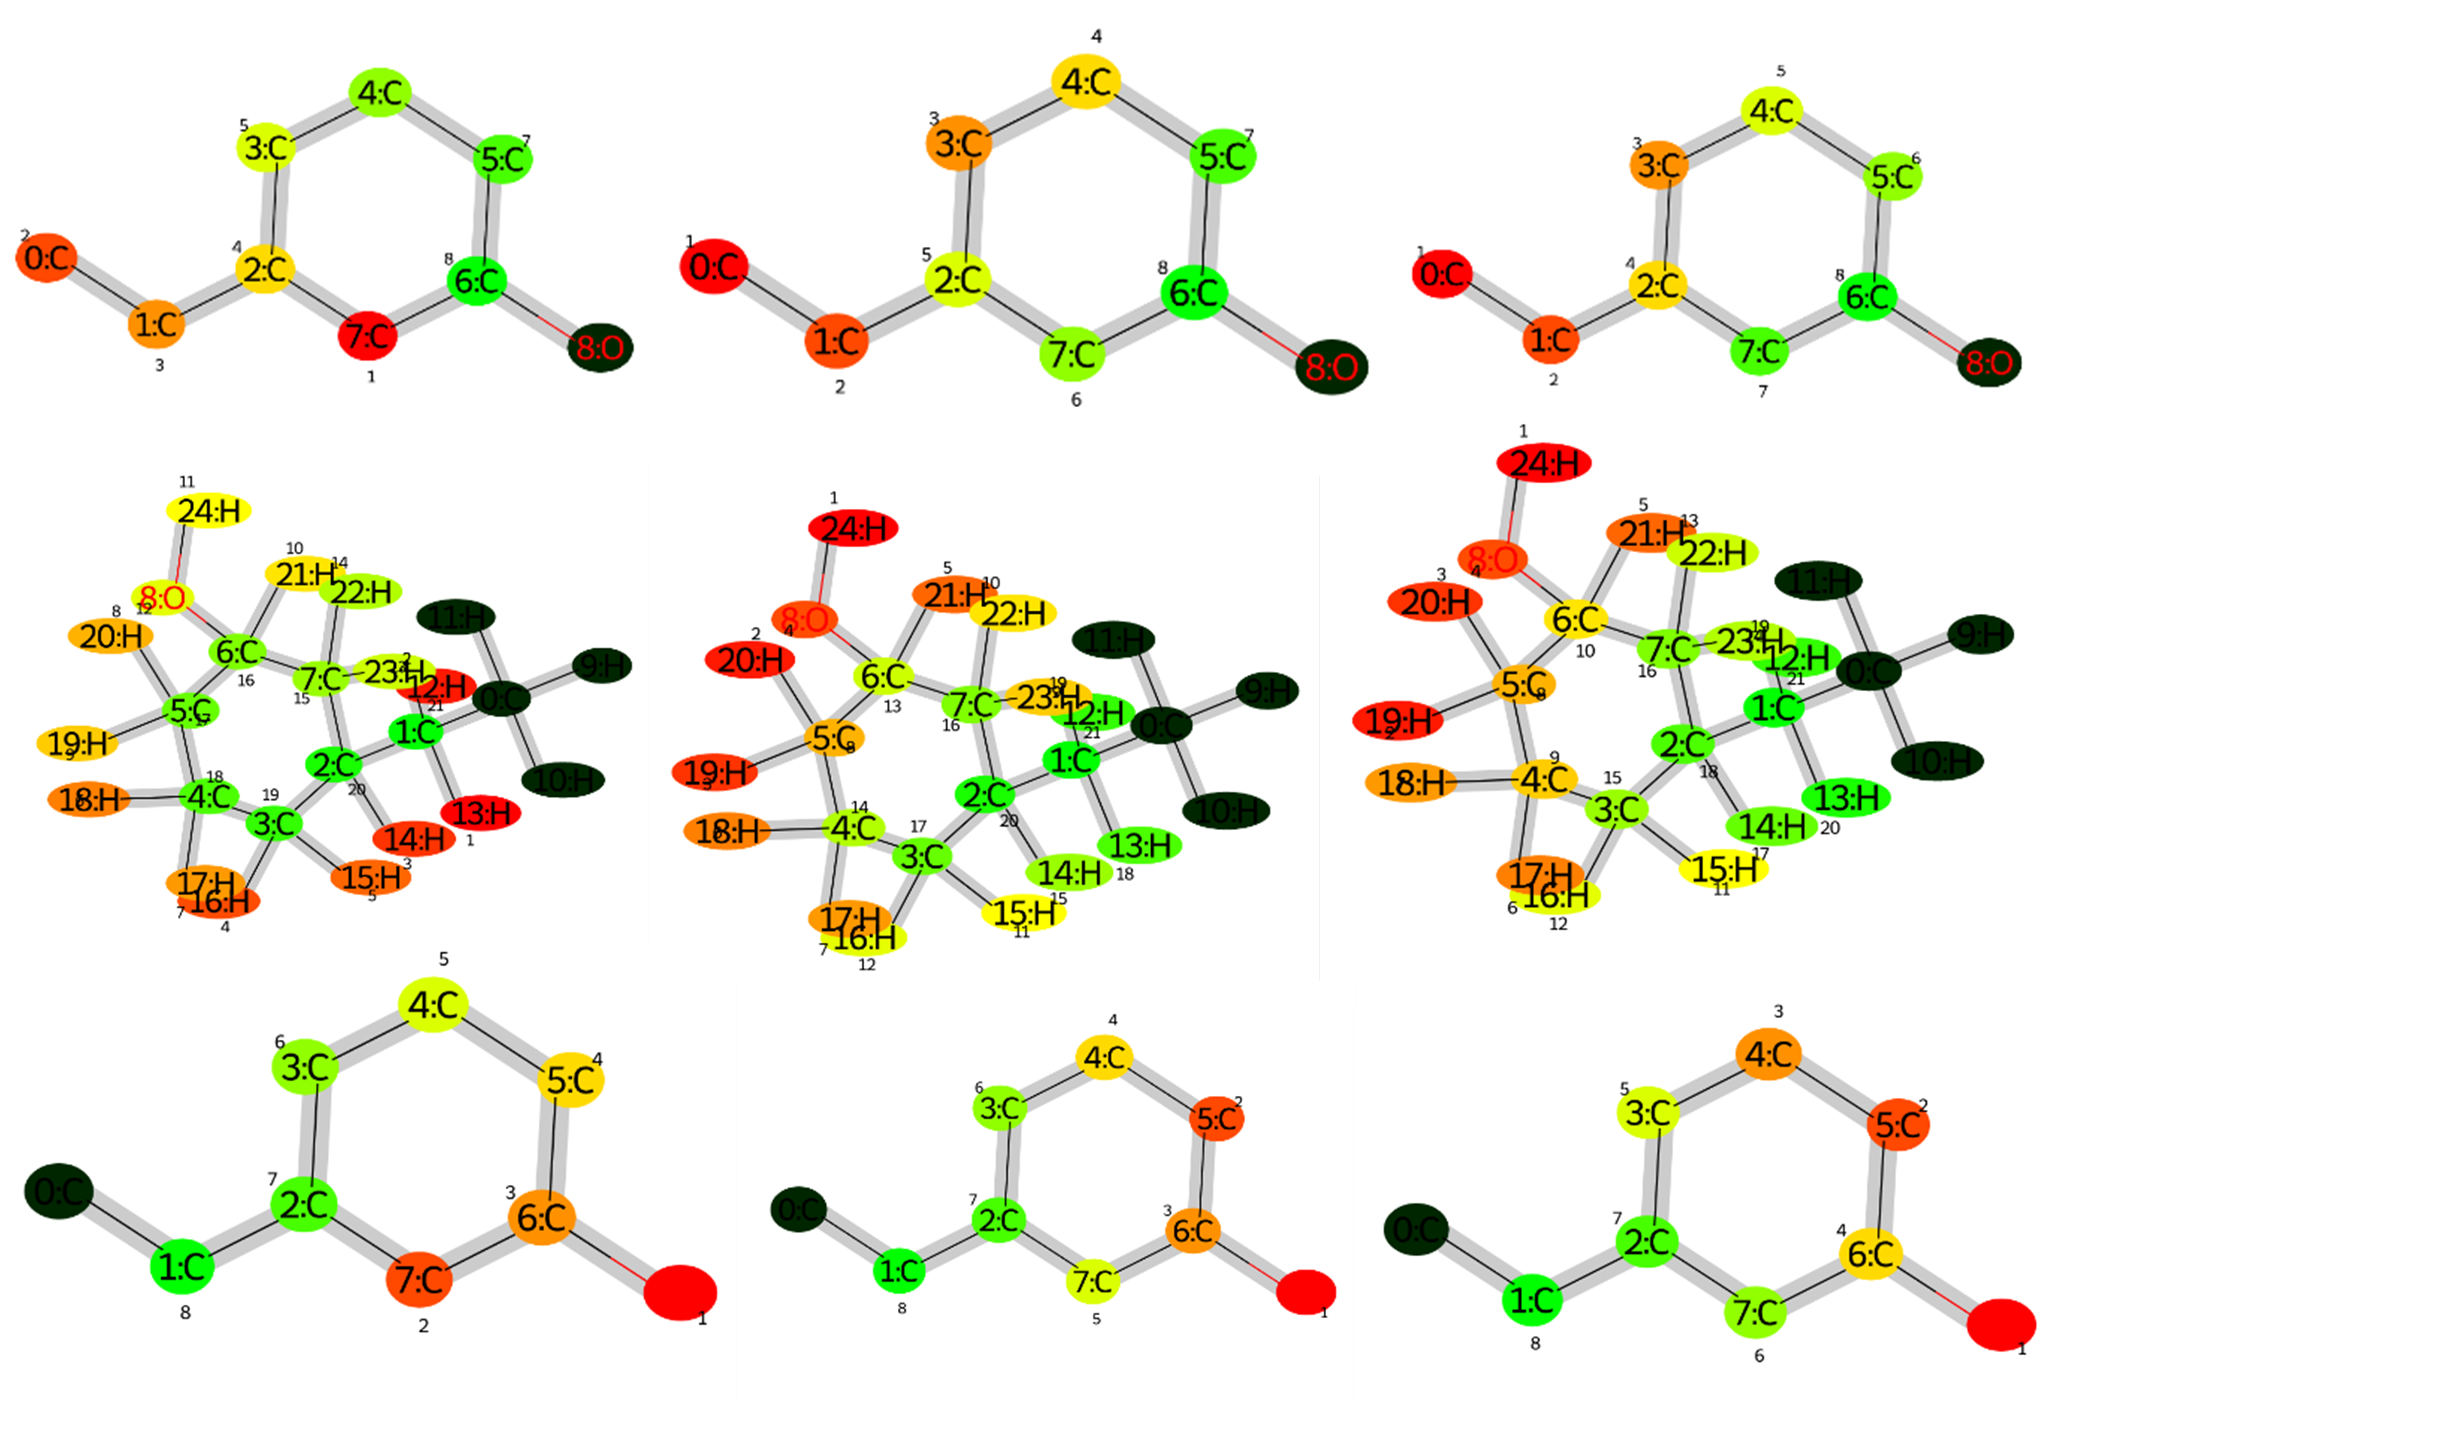
\includegraphics[scale=0.75]{ethylcyclohexane_set2}\caption{mutation route for ethylcyclohexane for ethylcyclohexane->methanol; first row: correct common core and mutation route, hydrogens excluded; middle row: hydrogens included; right: hydrogens included, but removed before drawing; left: DFS-algorithm; middle: BFS-algorithm; right: BFS-iter-algorithm; common core in dark, for these small molecules the differences between the new mutation algorithms (i.e. middle and right) are negligible}
	
\end{figure}

\begin{figure}[H]
	
	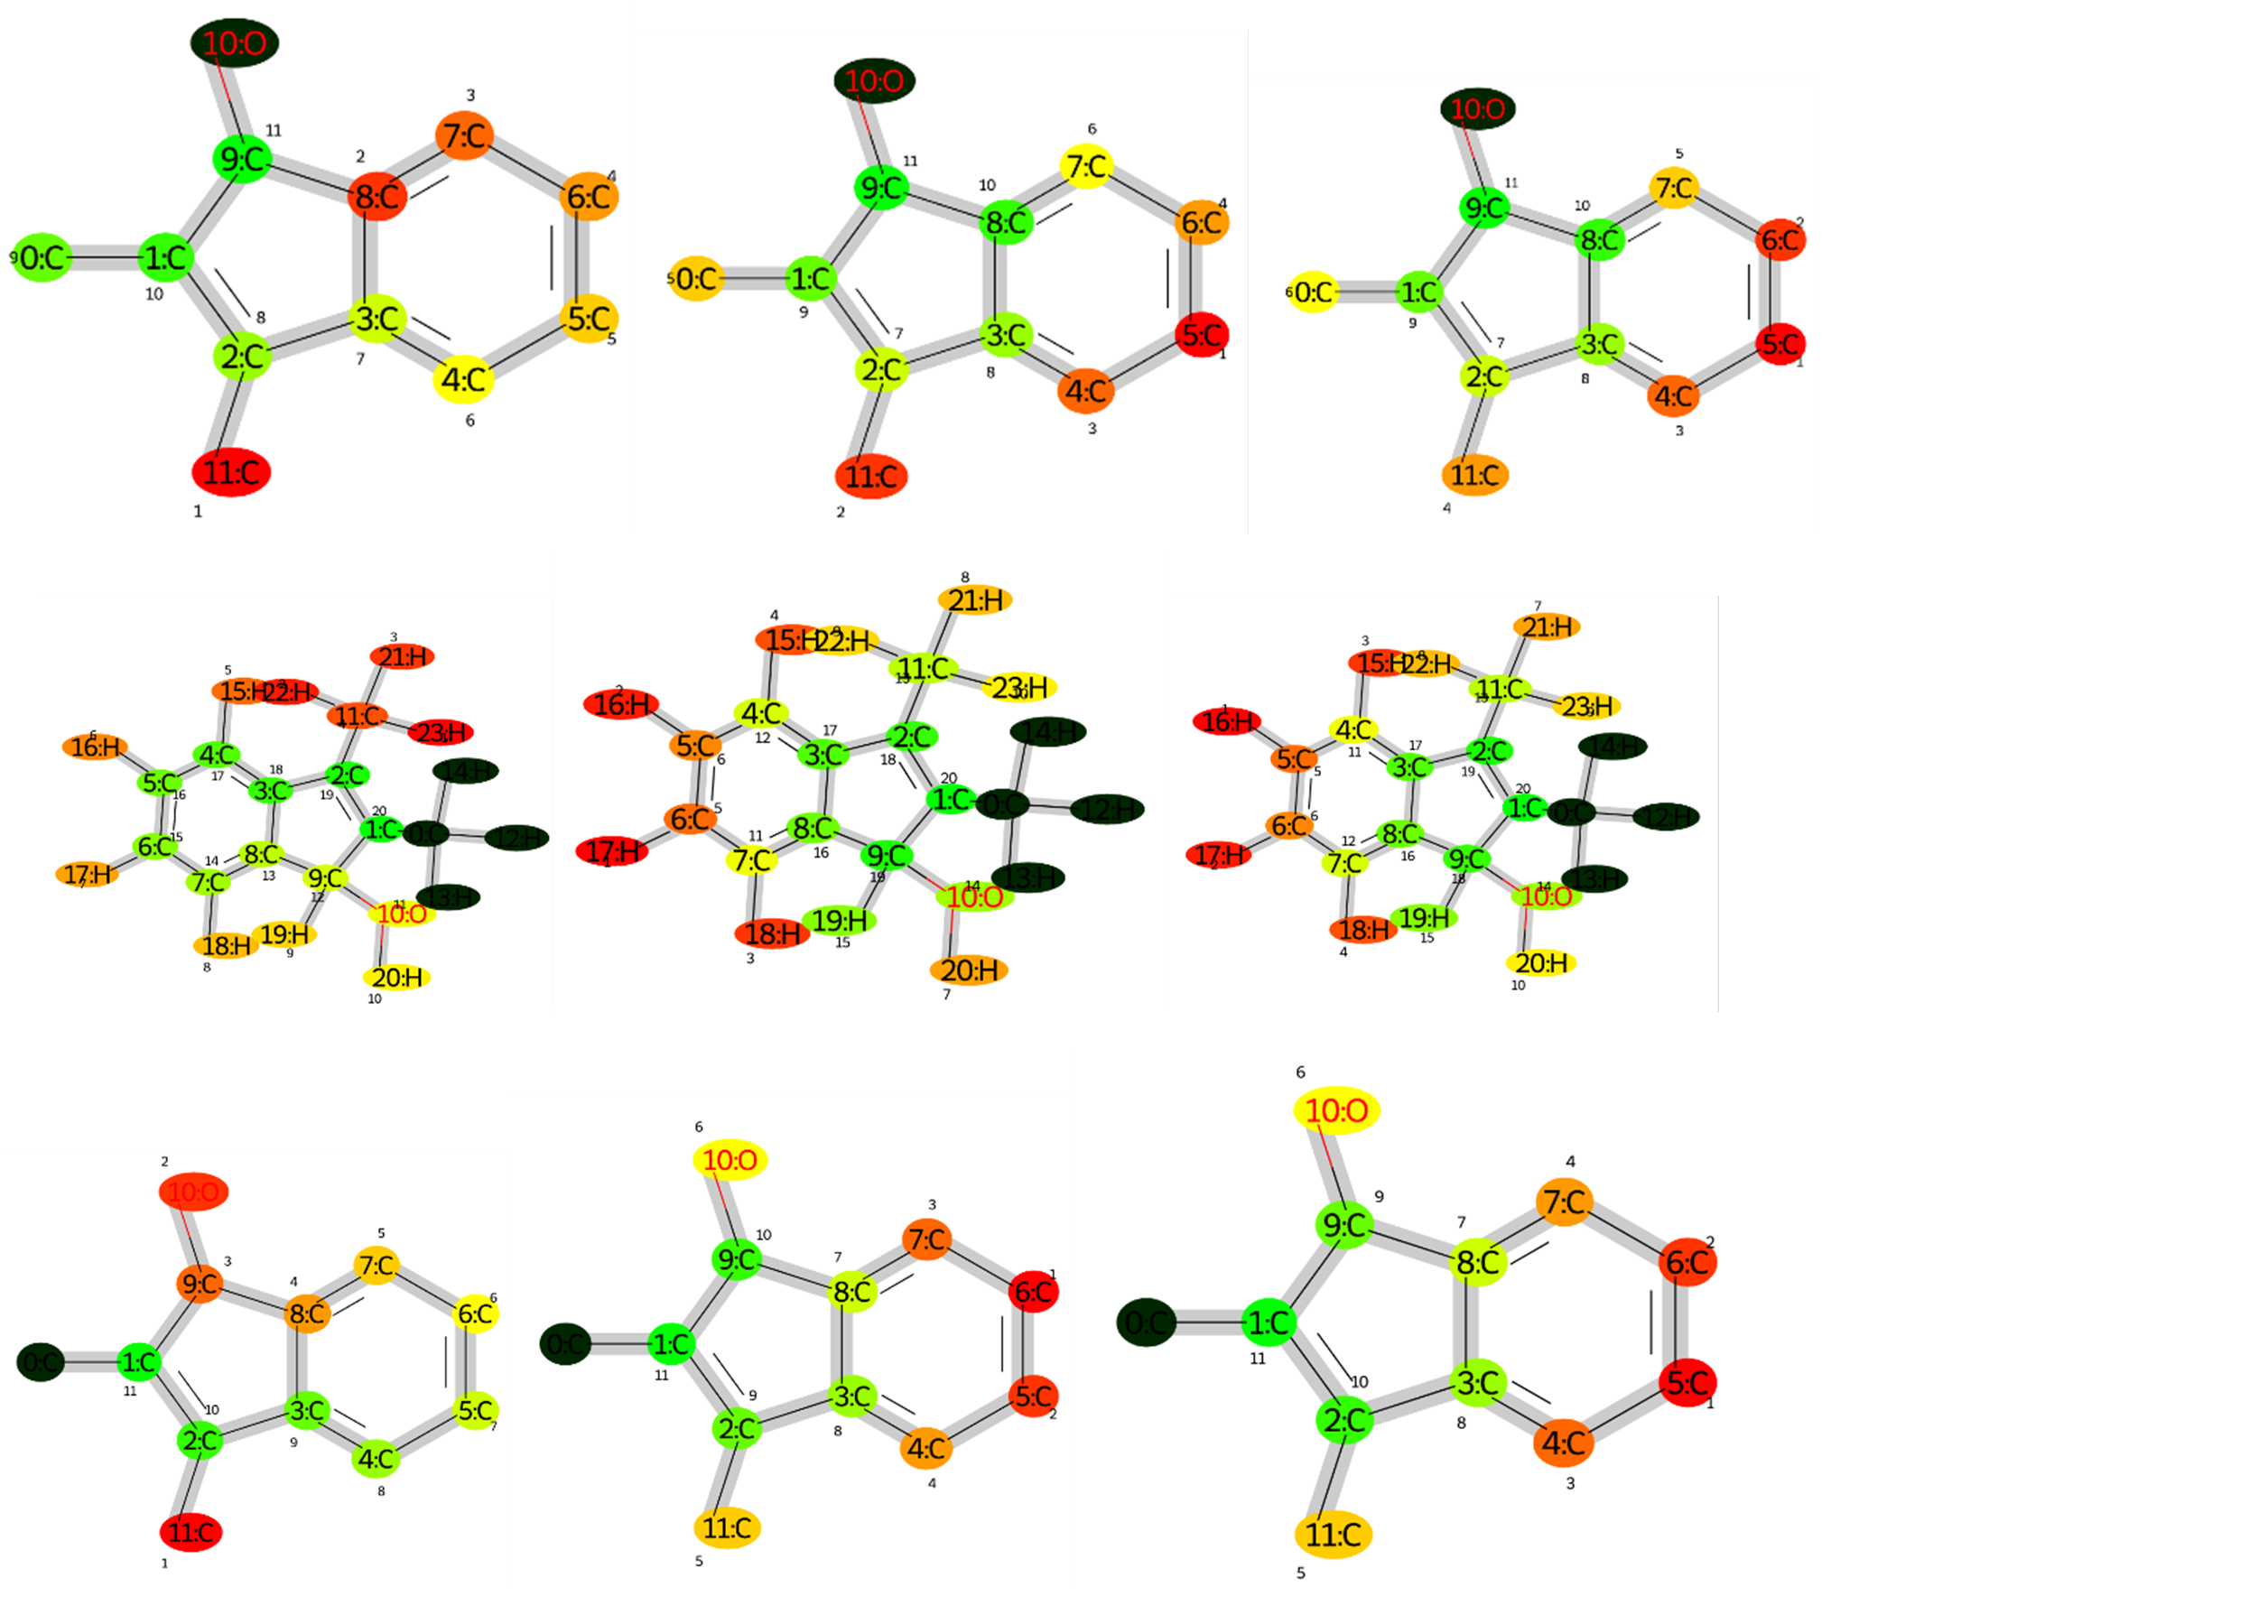
\includegraphics[scale=0.75]{dimethylindenol_set2}\caption{mutation route for dimethyl-inden-ol for dimethyl-inden-ol->methanol; first row: correct common core and mutation route, hydrogens excluded; middle row: hydrogens included; right: hydrogens included, but removed before drawing; left: DFS-algorithm; middle: BFS-algorithm; right: BFS-iter-algorithm; common core in dark, for these small molecules the differences between the new mutation algorithms (i.e. middle and right) are negligible}
	
\end{figure}

\section{Routes for molecules from Transformato paper}

\begin{figure}[!htb]
	
	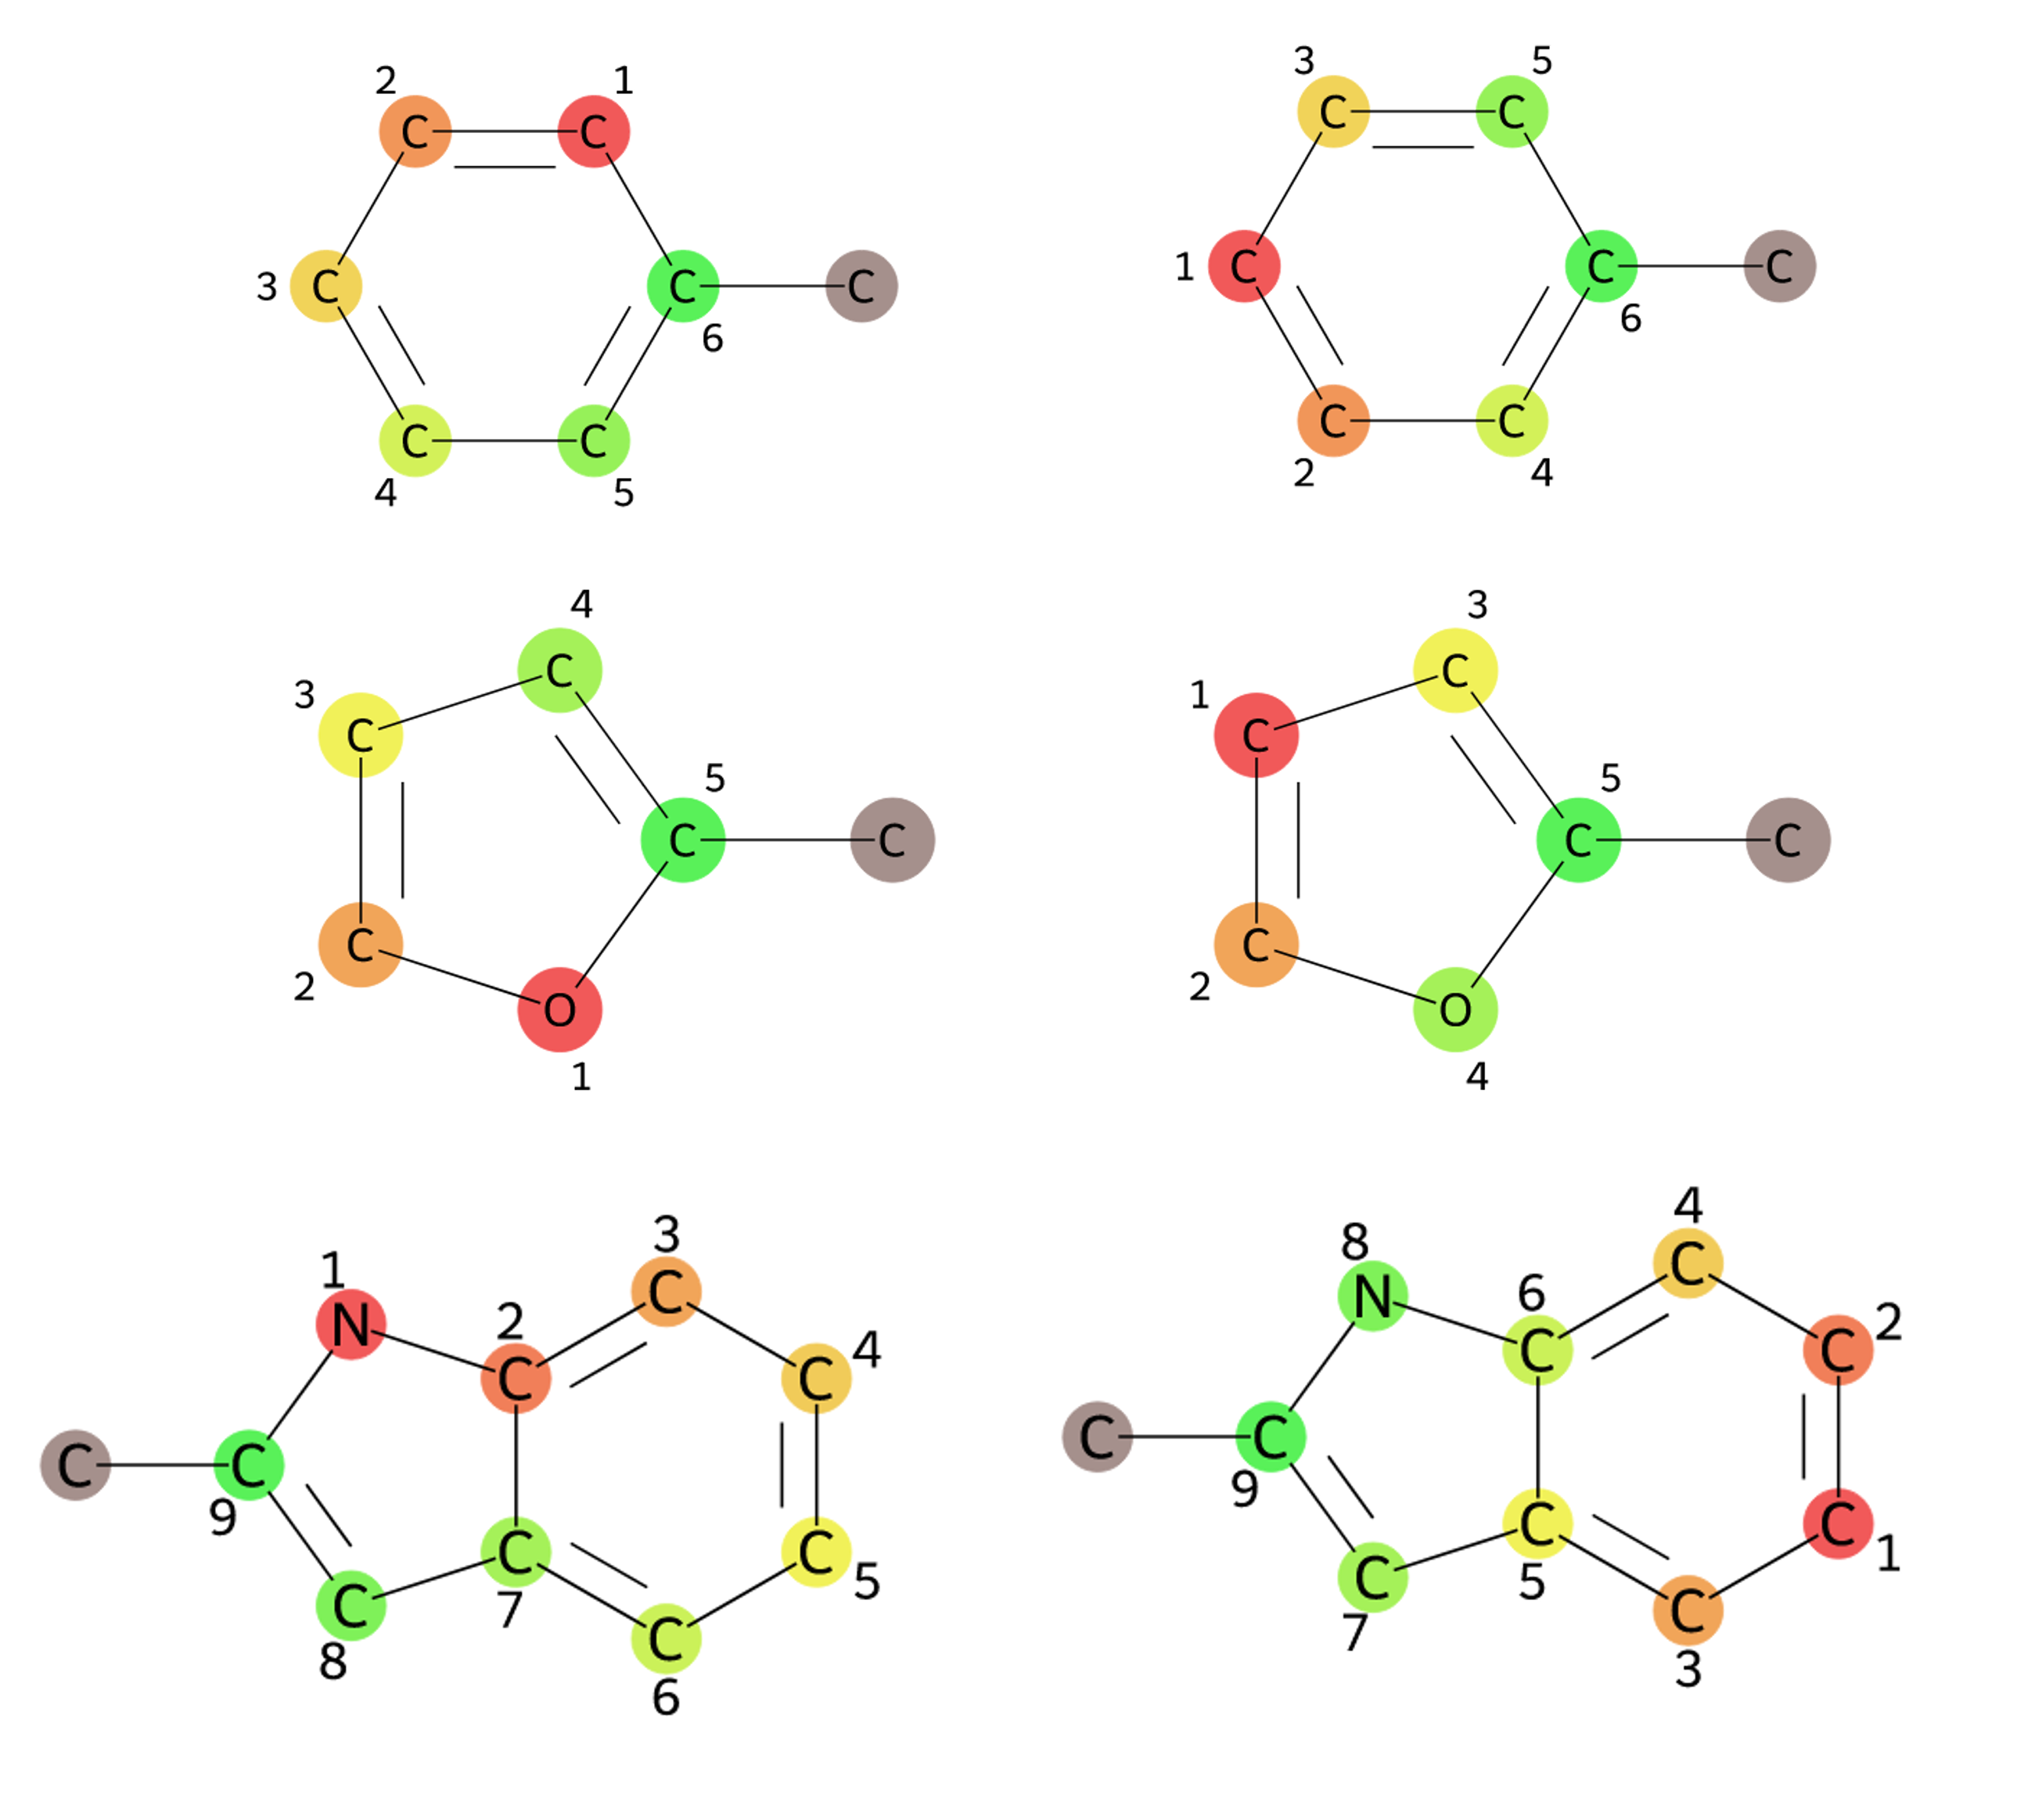
\includegraphics[scale=0.75]{paper_routes1a}\caption{left: DFS-algorithm; right: BFS--algorithm; common core in dark; from top to bottom row: mutation routes for toluene/methane, 2-methylfuran/methane, 2-methylindole/methane}
	
\end{figure}


\begin{figure}[!htb]
	
	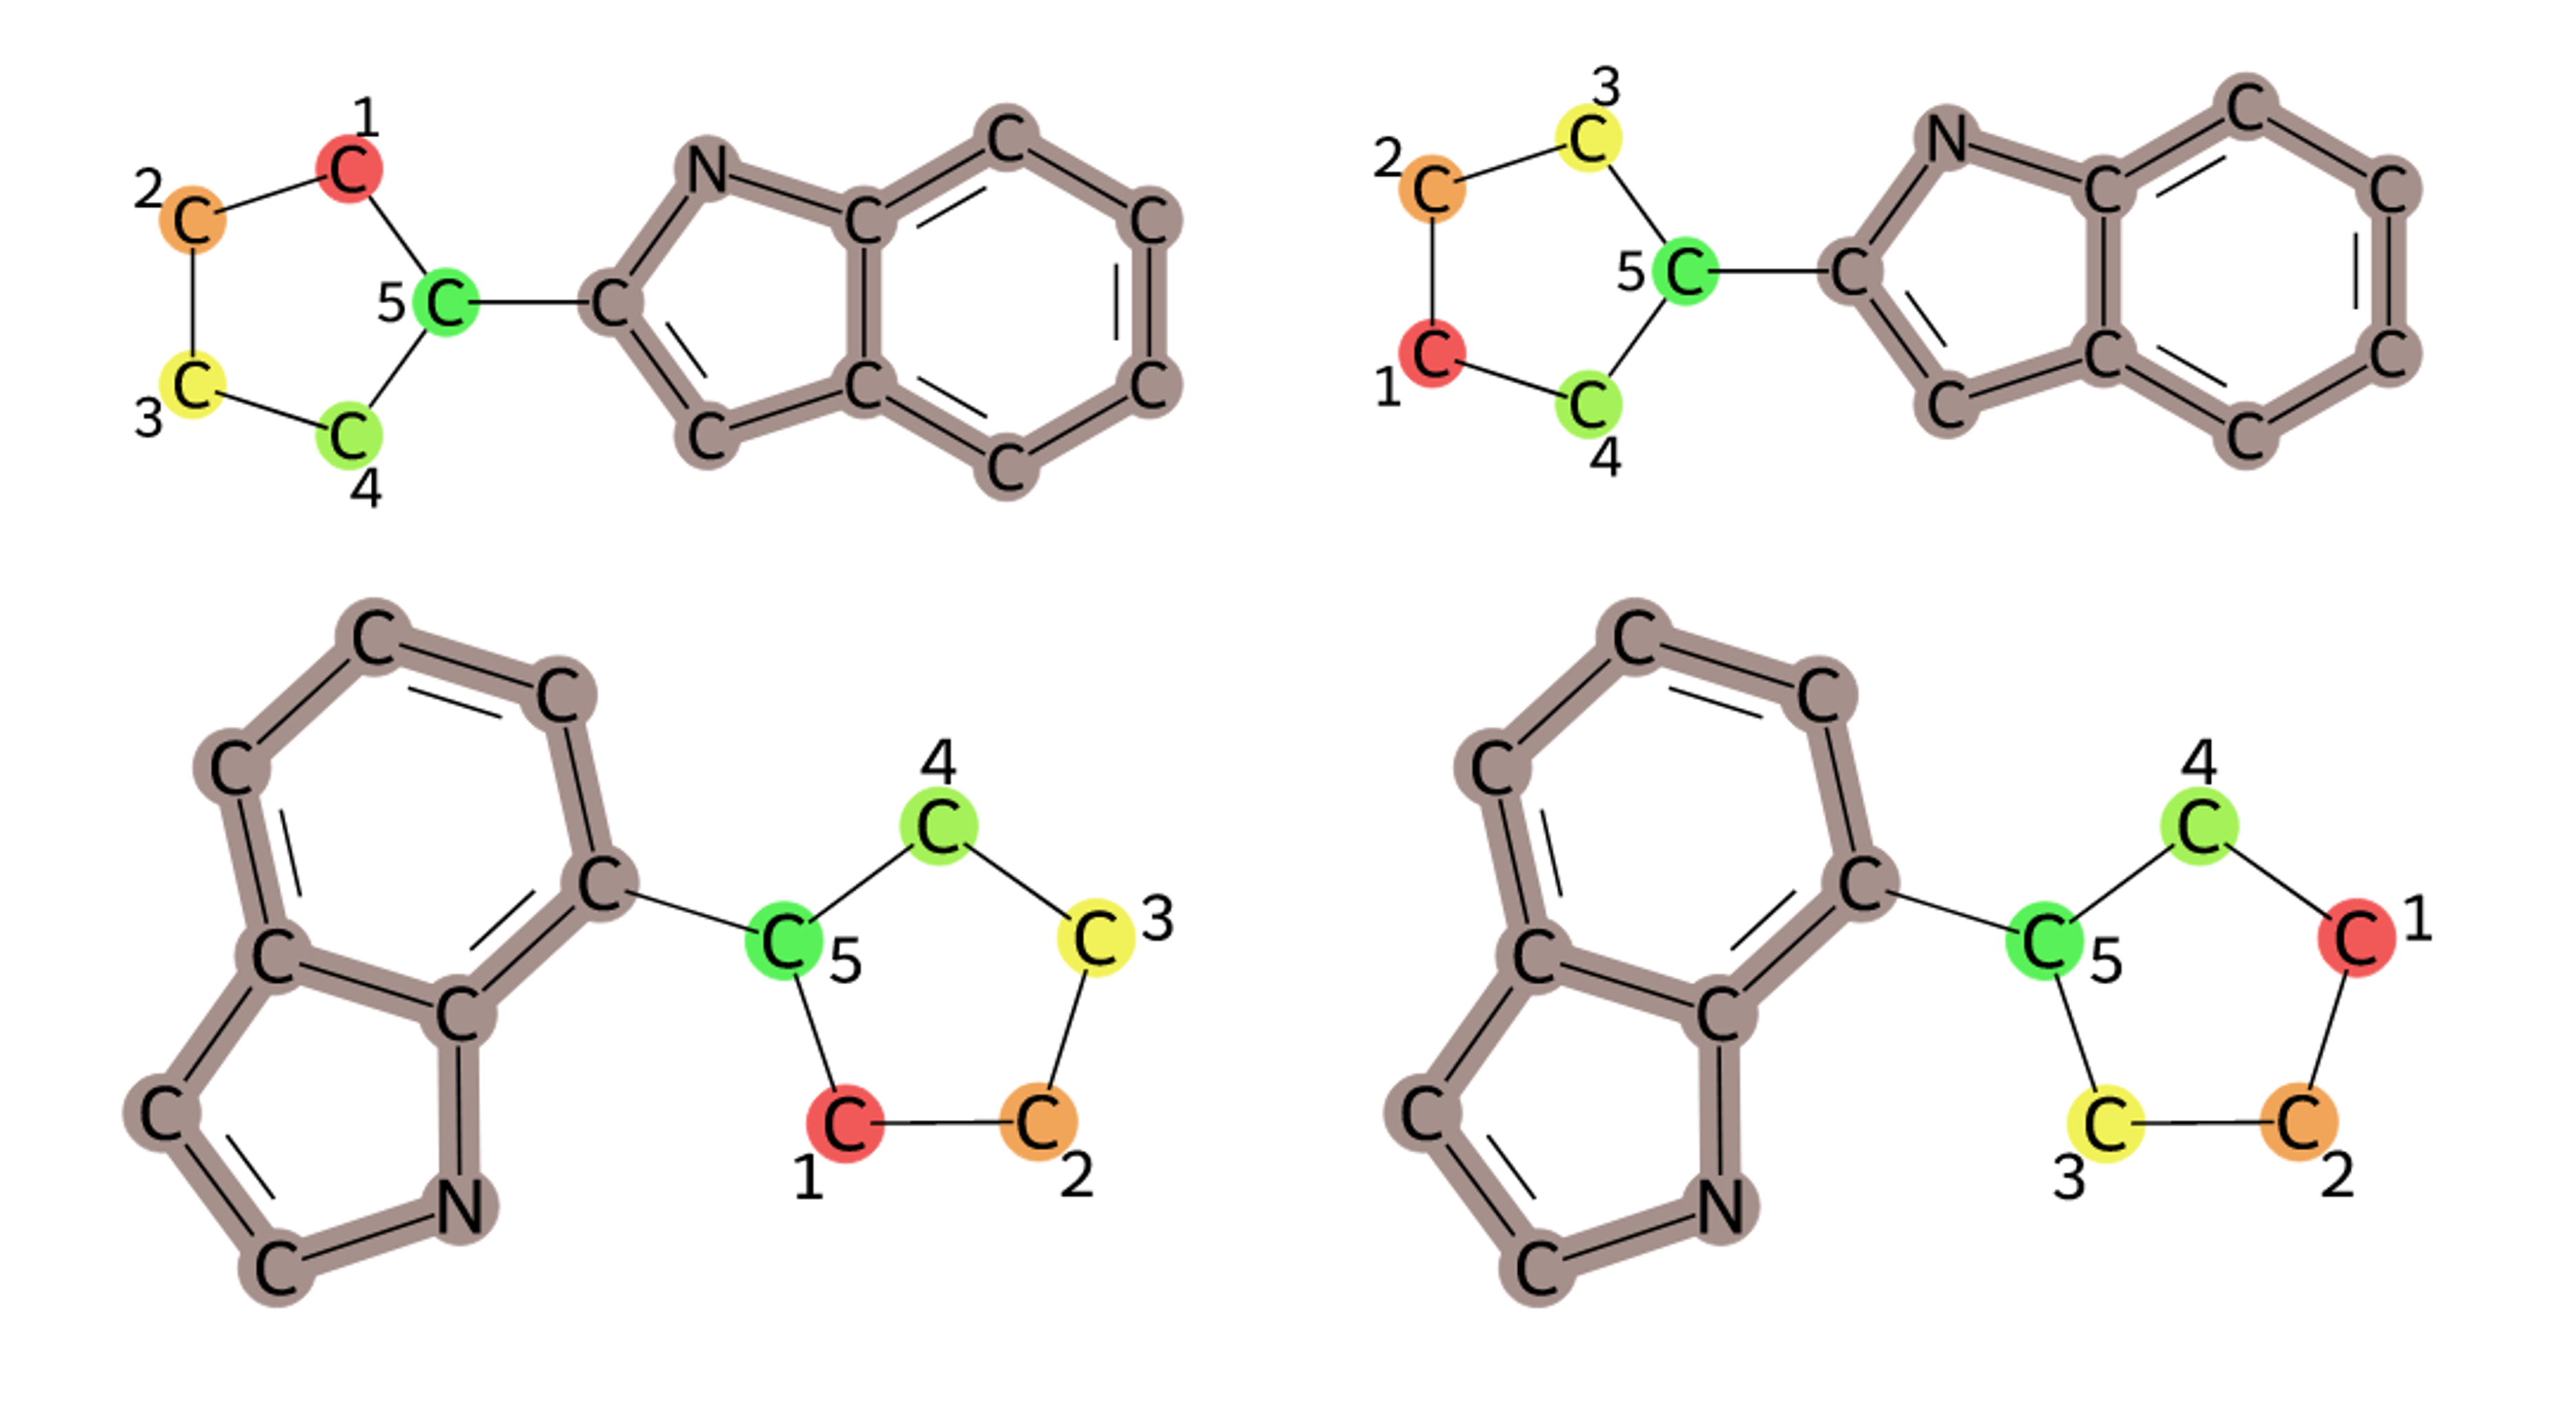
\includegraphics[scale=0.55]{paper_routes1b}\caption{left: DFS-algorithm; right: BFS-algorithm; common core in dark; mutation routes for 2-cyclopentylindole/7-cyclopentylindole}
	
\end{figure}


SMILES representations of the molecules used:


methane: C

Toluene: CC1=CC=CC=C1

2-Methylfuran: CC1=CC=CO1

methylindole2: CC1=CC2=CC=CC=C2N1

2-cyclopentylindole: C1CCC(C1)C1=CC2=CC=CC=C2N1

7-cyclopentylindole: C1CCC(C1)C1=C2NC=CC2=CC=C1





\section{Results for individual runs}

\begin{figure}[htp] 
	\centering
	\subfigure[Run 1]{%
		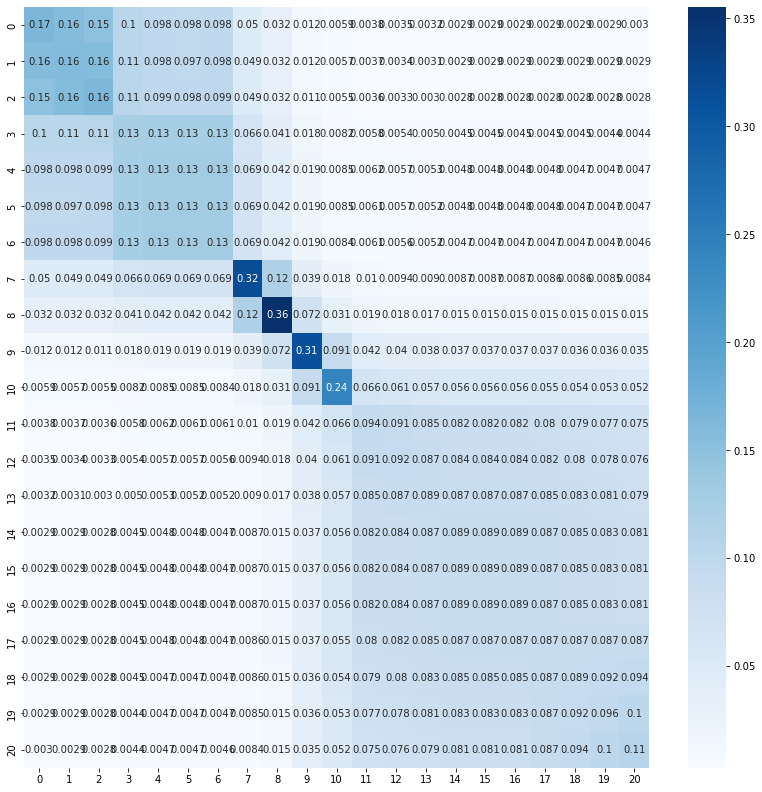
\includegraphics[width=0.4\textwidth]{naphthol_runs_old/vac_naphthol_overlap_old1}%
		\label{fig:v_naphthol_old11}%
	}\hfil
	\subfigure[Run 2]{%
		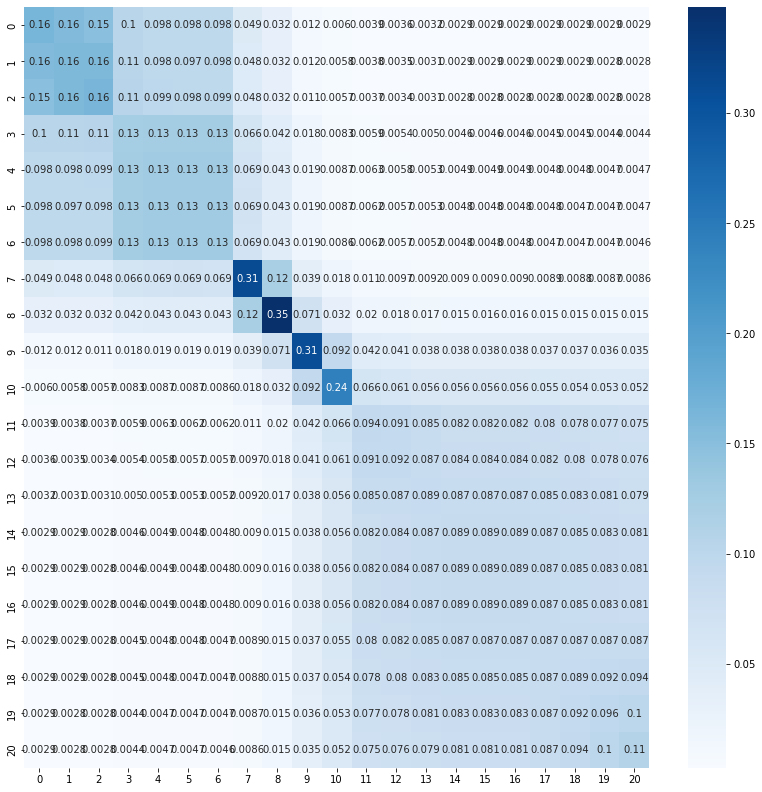
\includegraphics[width=0.4\textwidth]{naphthol_runs_old/vac_naphthol_overlap_old2}%
		\label{fig:v_naphthol_new12}%
	}
	
	\subfigure[Run 3]{%
		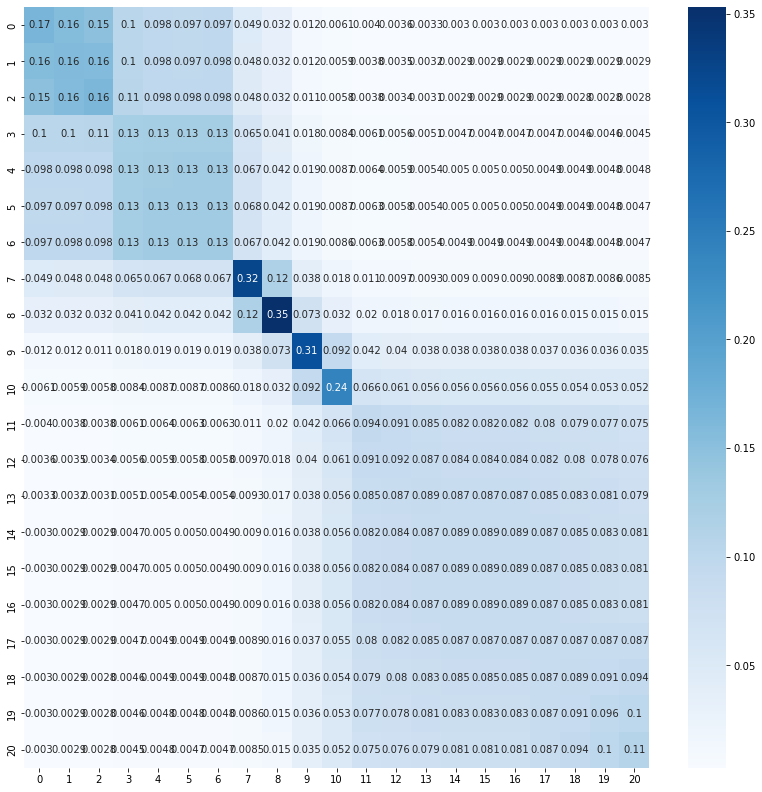
\includegraphics[width=0.4\textwidth]{naphthol_runs_old/vac_naphthol_overlap_old3}%
		\label{fig:w_naphthol_old13}%
	}\hfil
	\subfigure[Run 4]{%
		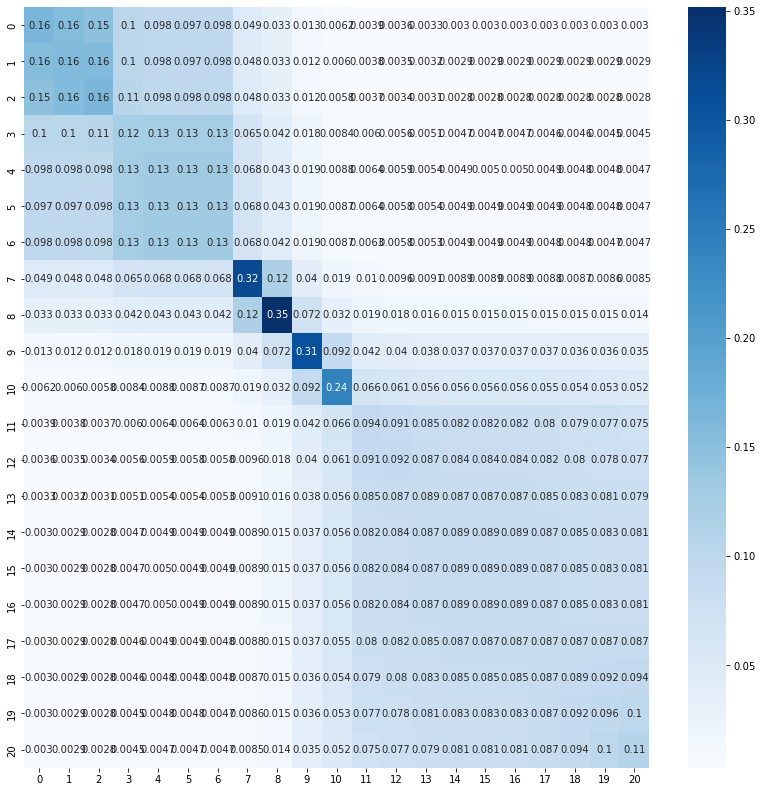
\includegraphics[width=0.4\textwidth]{naphthol_runs_old/vac_naphthol_overlap_old4}%
		\label{fig:w_napthol_new14}%
	}
	
	\caption{Overlap plots for Naphthol/Vacuum, old algorithm}
\end{figure}


\begin{figure}[htp] 
	\centering
	\subfigure[Run 1]{%
		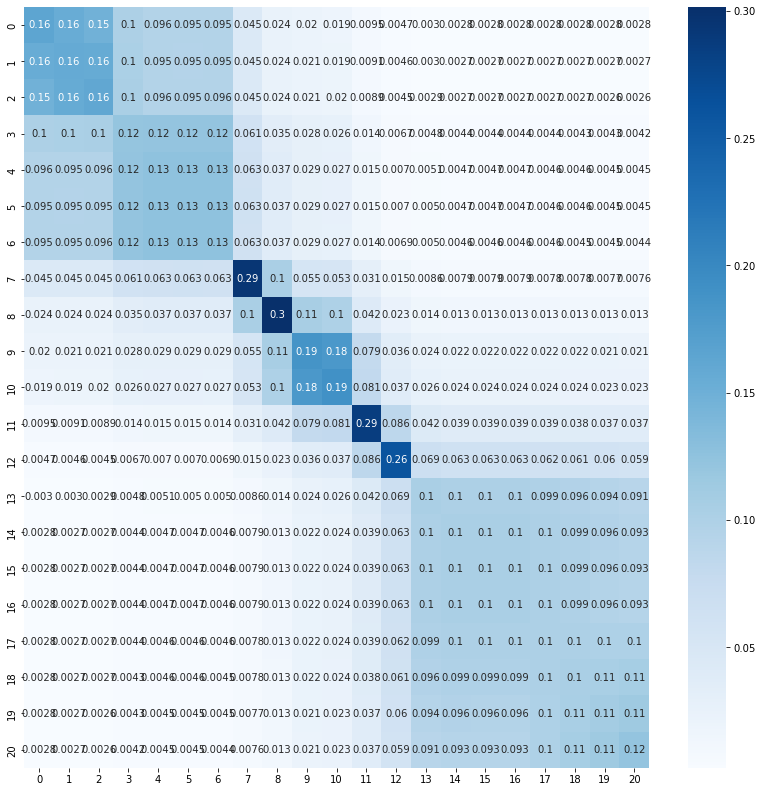
\includegraphics[width=0.4\textwidth]{naphthol_runs_new/vac_naphthol_overlap_new1}%
		\label{fig:naphtvacnew1}%
	}\hfil
	\subfigure[Run 2]{%
		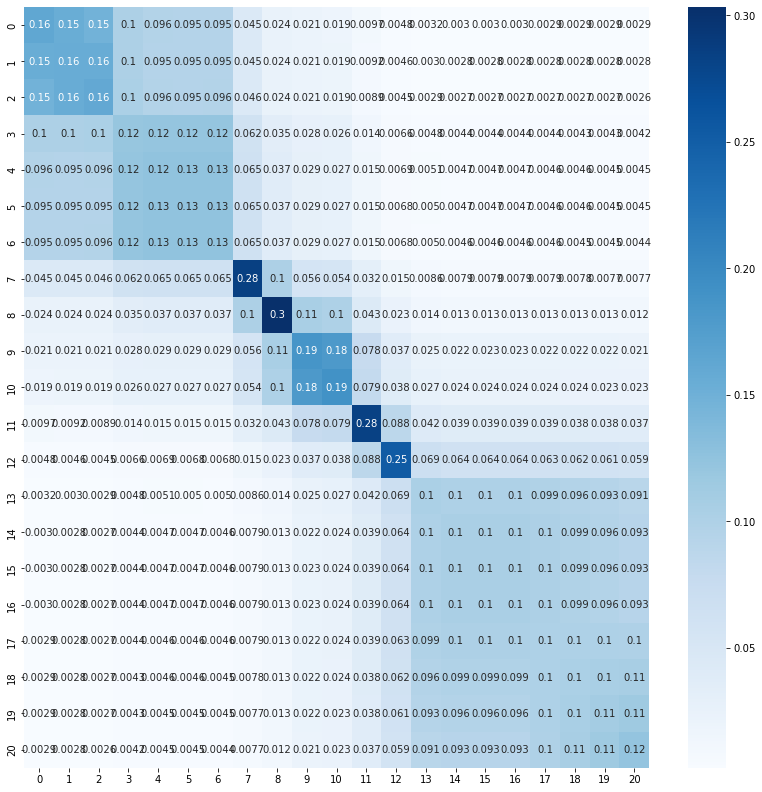
\includegraphics[width=0.4\textwidth]{naphthol_runs_new/vac_naphthol_overlap_new2}%
		\label{fig:naphtvacnew2}%
	}
	
	\subfigure[Run 3]{%
		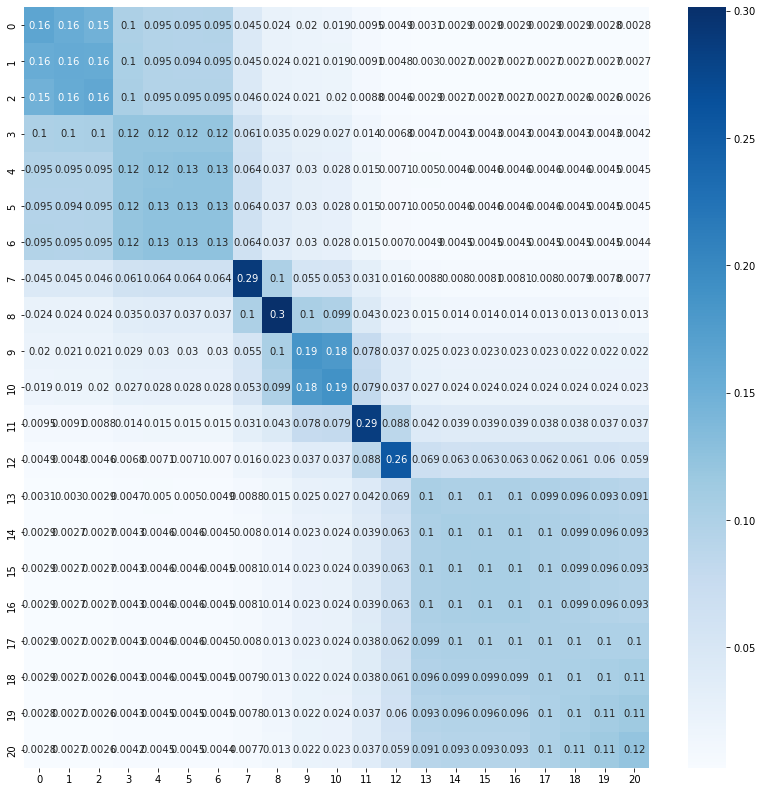
\includegraphics[width=0.4\textwidth]{naphthol_runs_new/vac_naphthol_overlap_new3}%
		\label{fig:naphtvacnew3}%
	}\hfil
	\subfigure[Run 4]{%
		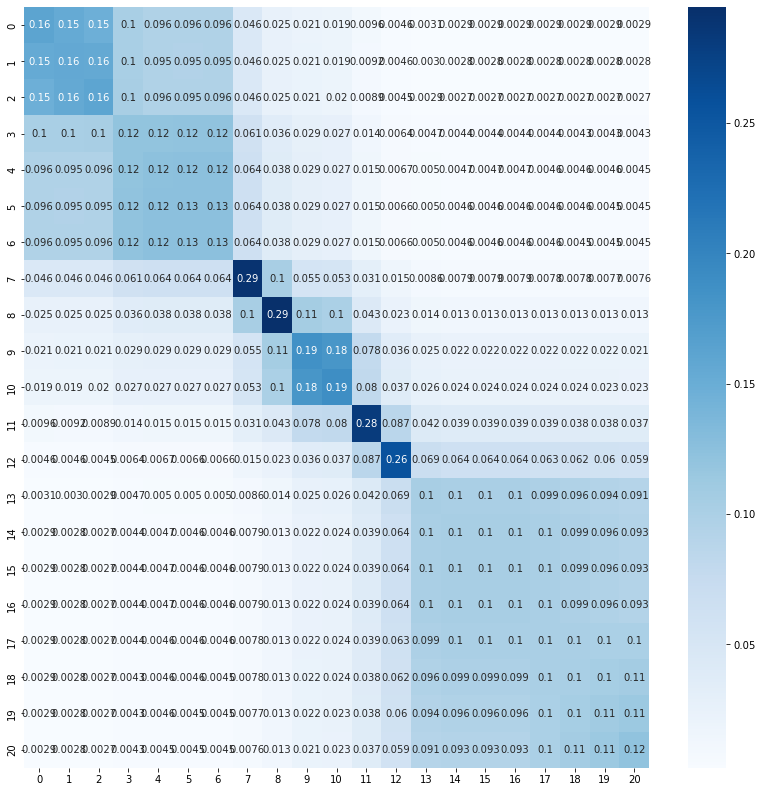
\includegraphics[width=0.4\textwidth]{naphthol_runs_new/vac_naphthol_overlap_new4}%
		\label{fig:naphtvacnew4}%
	}
	
	\caption{Overlap plots for Naphthol/Vacuum, new algorithm}
\end{figure}


\begin{figure}[htp] 
	\centering
	\subfigure[Run 1]{%
		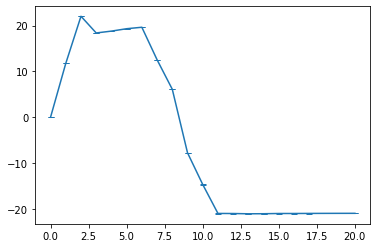
\includegraphics[width=0.4\textwidth]{naphthol_runs_old/vac_naphthol_states_old1}%
		\label{fig:v_naphthol_old11states}%
	}\hfil
	\subfigure[Run 2]{%
		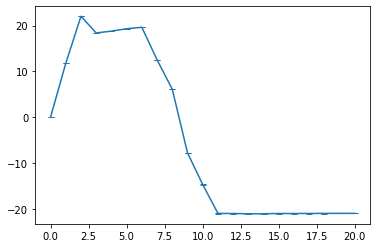
\includegraphics[width=0.4\textwidth]{naphthol_runs_old/vac_naphthol_states_old2}%
		\label{fig:v_naphthol_new12states}%
	}
	
	\subfigure[Run 3]{%
		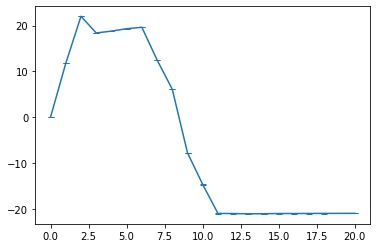
\includegraphics[width=0.4\textwidth]{naphthol_runs_old/vac_naphthol_states_old3}%
		\label{fig:w_naphthol_old13states}%
	}\hfil
	\subfigure[Run 4]{%
		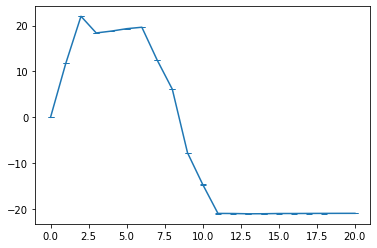
\includegraphics[width=0.4\textwidth]{naphthol_runs_old/vac_naphthol_states_old4}%
		\label{fig:w_napthol_new14states}%
	}
	
	\caption{Lambda states for Naphthol/Vacuum, old algorithm}
\end{figure}



\begin{figure}[htp] 
	\centering
	\subfigure[Run 1]{%
		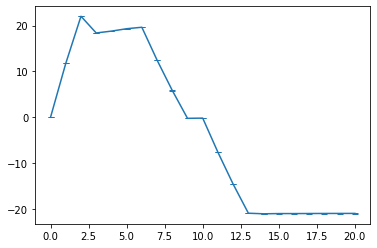
\includegraphics[width=0.4\textwidth]{naphthol_runs_new/vac_naphthol_states_new1}%
		\label{fig:naphtvacnew1states}%
	}\hfil
	\subfigure[Run 2]{%
		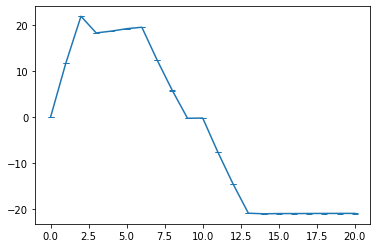
\includegraphics[width=0.4\textwidth]{naphthol_runs_new/vac_naphthol_states_new2}%
		\label{fig:naphtvacnew2states}%
	}
	
	\subfigure[Run 3]{%
		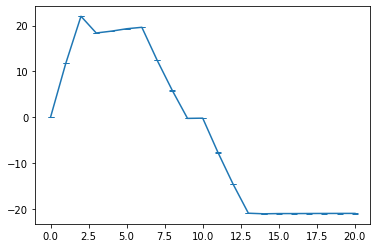
\includegraphics[width=0.4\textwidth]{naphthol_runs_new/vac_naphthol_states_new3}%
		\label{fig:naphtvacnew3states}%
	}\hfil
	\subfigure[Run 4]{%
		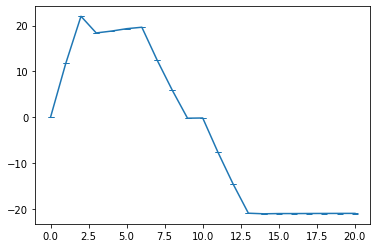
\includegraphics[width=0.4\textwidth]{naphthol_runs_new/vac_naphthol_states_new4}%
		\label{fig:naphtvacnew4states}%
	}
	
	\caption{Lambda states for Naphthol/Vacuum, new algorithm}
\end{figure}








\begin{figure}[htp] 
	\centering
	\subfigure[Run 1]{%
		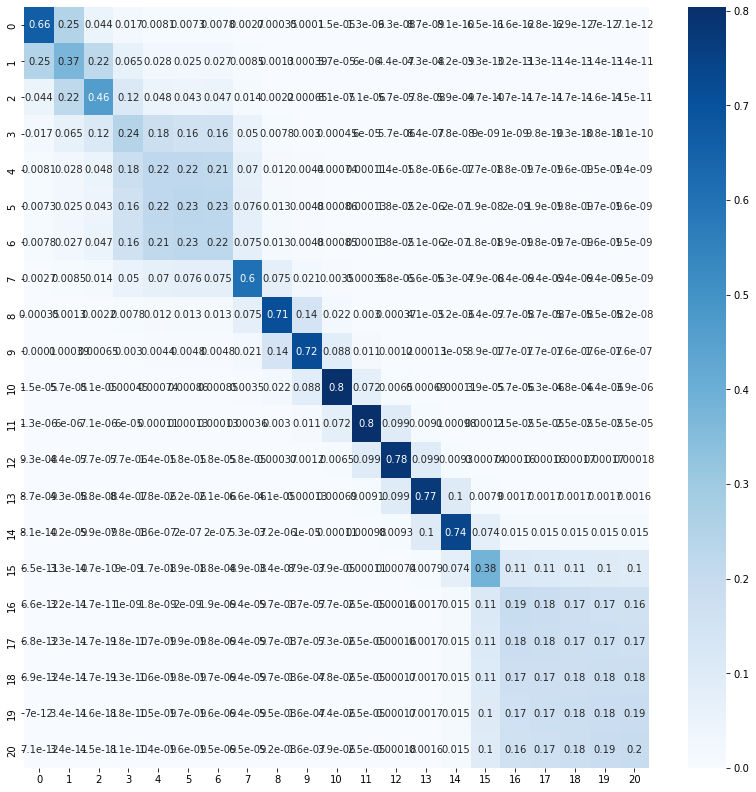
\includegraphics[width=0.4\textwidth]{naphthol_runs_old/waterbox_naphthol_overlap_old1}%
		\label{fig:v_naphthol_old11}%
	}\hfil
	\subfigure[Run 2]{%
		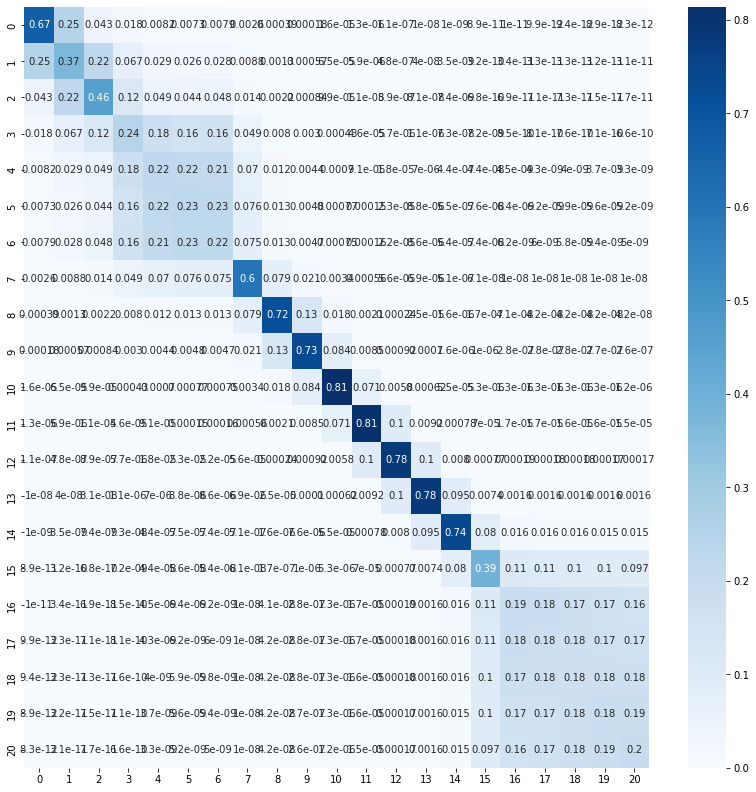
\includegraphics[width=0.4\textwidth]{naphthol_runs_old/waterbox_naphthol_overlap_old2}%
		\label{fig:v_naphthol_new12}%
	}
	
	\subfigure[Run 3]{%
		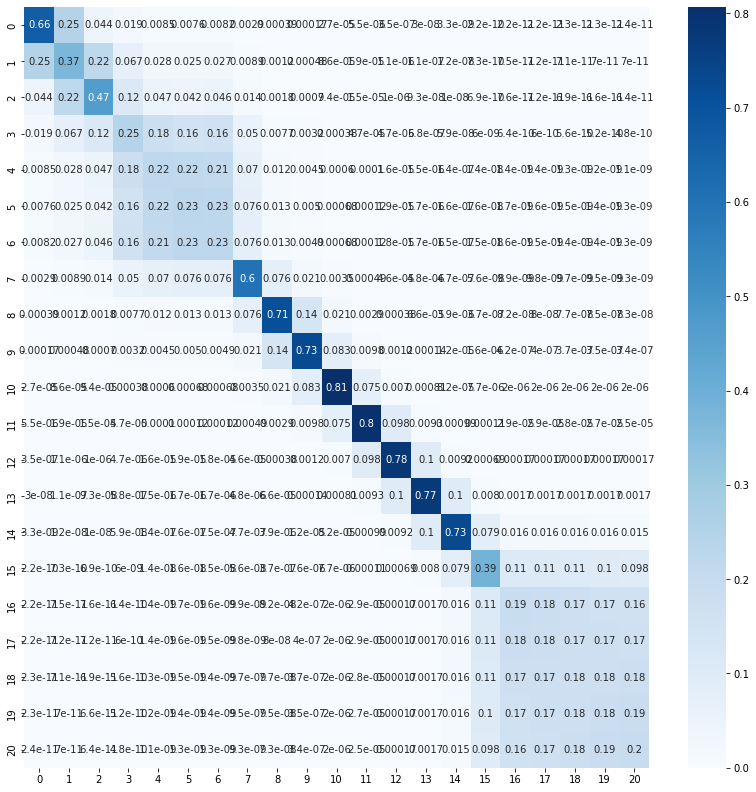
\includegraphics[width=0.4\textwidth]{naphthol_runs_old/waterbox_naphthol_overlap_old3}%
		\label{fig:w_naphthol_old13}%
	}\hfil
	\subfigure[Run 4]{%
		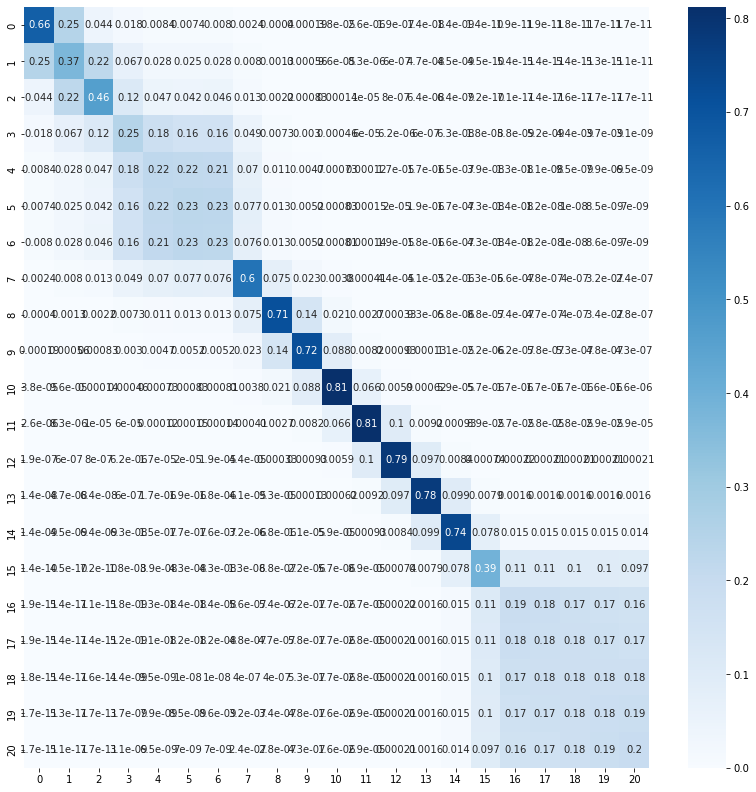
\includegraphics[width=0.4\textwidth]{naphthol_runs_old/waterbox_naphthol_overlap_old4}%
		\label{fig:w_napthol_new14}%
	}
	
	\caption{Overlap plots for Naphthol/Waterbox, old algorithm}
\end{figure}


\begin{figure}[htp] 
	\centering
	\subfigure[Run 1]{%
		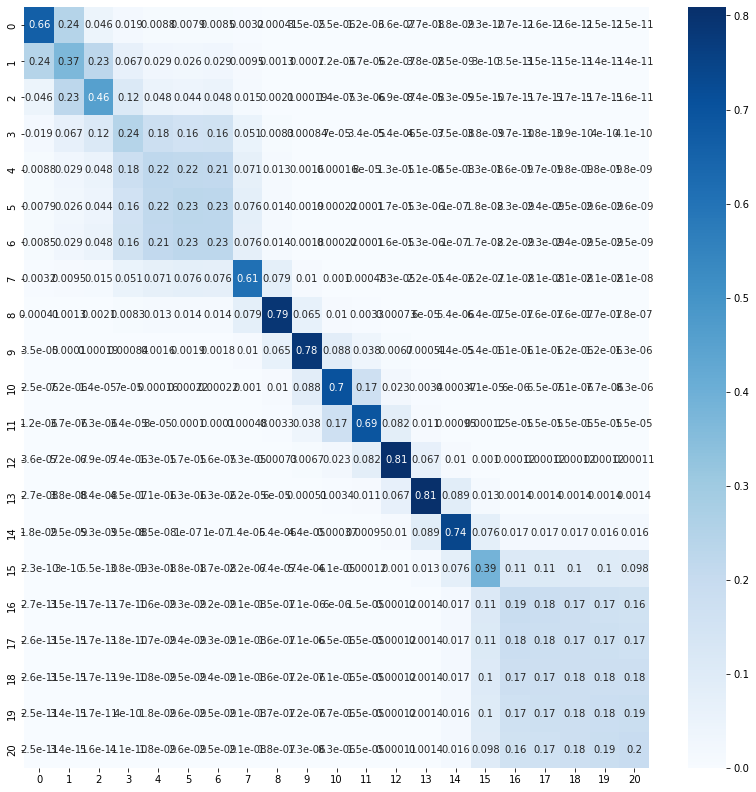
\includegraphics[width=0.4\textwidth]{naphthol_runs_new/waterbox_naphthol_overlap_new1}%
		\label{fig:naphtwatnew1}%
	}\hfil
	\subfigure[Run 2]{%
		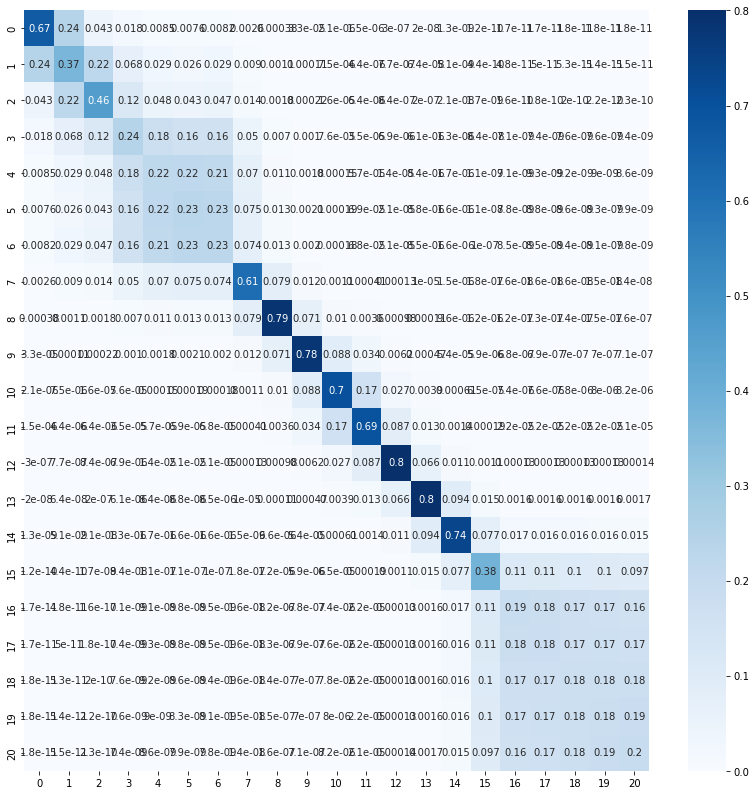
\includegraphics[width=0.4\textwidth]{naphthol_runs_new/waterbox_naphthol_overlap_new2}%
		\label{fig:naphtwatnew2}%
	}
	
	\subfigure[Run 3]{%
		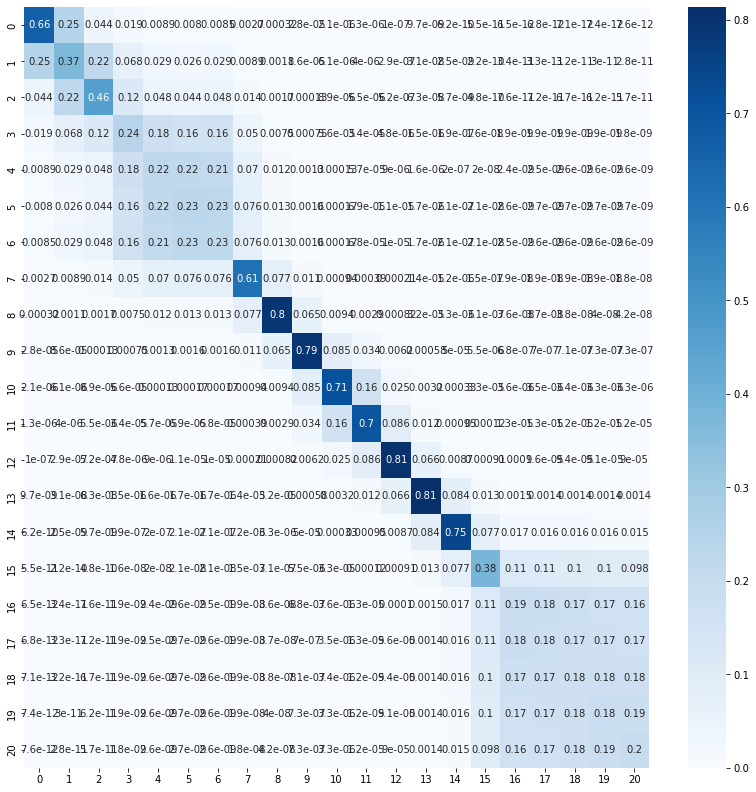
\includegraphics[width=0.4\textwidth]{naphthol_runs_new/waterbox_naphthol_overlap_new3}%
		\label{fig:naphtwatnew3}%
	}\hfil
	\subfigure[Run 4]{%
		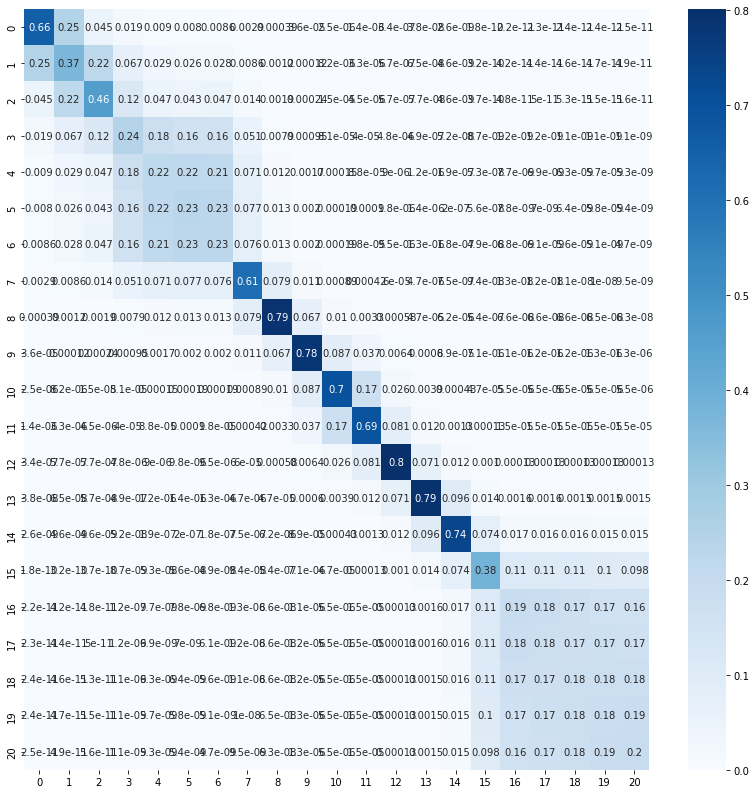
\includegraphics[width=0.4\textwidth]{naphthol_runs_new/waterbox_naphthol_overlap_new4}%
		\label{fig:naphtwatnew4}%
	}
	
	\caption{Overlap plots for Naphthol/Waterbox, new algorithm}
\end{figure}



\begin{figure}[htp] 
	\centering
	\subfigure[Run 1]{%
		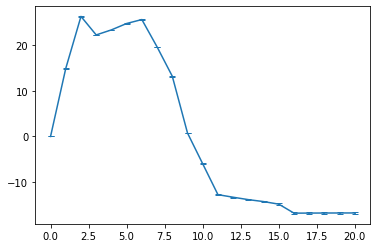
\includegraphics[width=0.4\textwidth]{naphthol_runs_old/waterbox_naphthol_states_old1}%
		\label{fig:v_naphthol_old11statess}%
	}\hfil
	\subfigure[Run 2]{%
		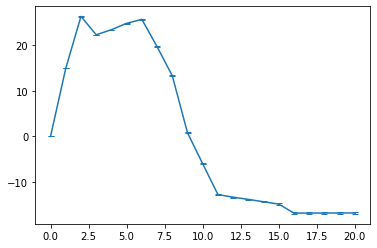
\includegraphics[width=0.4\textwidth]{naphthol_runs_old/waterbox_naphthol_states_old2}%
		\label{fig:v_naphthol_new12statess}%
	}
	
	\subfigure[Run 3]{%
		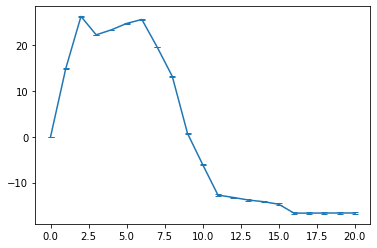
\includegraphics[width=0.4\textwidth]{naphthol_runs_old/waterbox_naphthol_states_old3}%
		\label{fig:w_naphthol_old13statess}%
	}\hfil
	\subfigure[Run 4]{%
		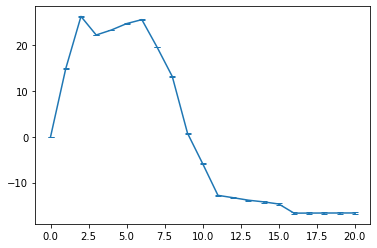
\includegraphics[width=0.4\textwidth]{naphthol_runs_old/waterbox_naphthol_states_old4}%
		\label{fig:w_napthol_new14statess}%
	}
	
	\caption{Lambda states for Naphthol/Waterbox, old algorithm}
\end{figure}


\begin{figure}[htp]
	\centering
	\subfigure[Run 1]{%
		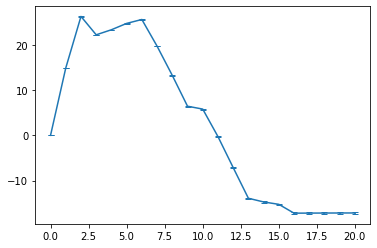
\includegraphics[width=0.4\textwidth]{naphthol_runs_new/waterbox_naphthol_states_new1}%
		\label{fig:naphtwatnew1states}%
	}\hfil
	\subfigure[Run 2]{%
		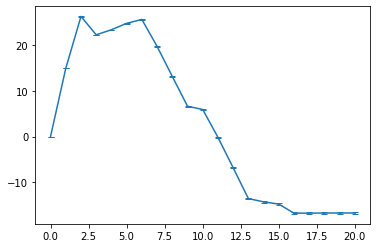
\includegraphics[width=0.4\textwidth]{naphthol_runs_new/waterbox_naphthol_states_new2}%
		\label{fig:naphtwatnew2states}%
	}
	
	\subfigure[Run 3]{%
		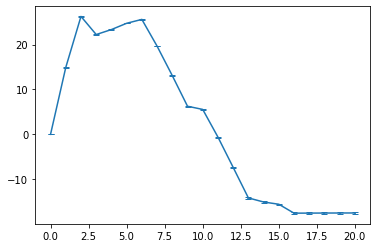
\includegraphics[width=0.4\textwidth]{naphthol_runs_new/waterbox_naphthol_states_new3}%
		\label{fig:naphtwatnew3states}%
	}\hfil
	\subfigure[Run 4]{%
		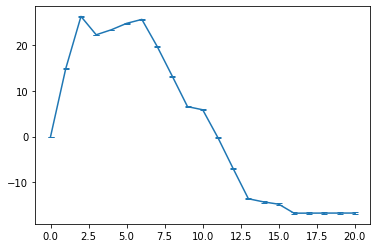
\includegraphics[width=0.4\textwidth]{naphthol_runs_new/waterbox_naphthol_states_new4}%
		\label{fig:naphtwatnew4states}%
	}
	
	\caption{Lambda states for Naphthol/Waterbox, new algorithm}
\end{figure}


\begin{figure}[htp] 
	\centering
	\subfigure[Run 1]{%
		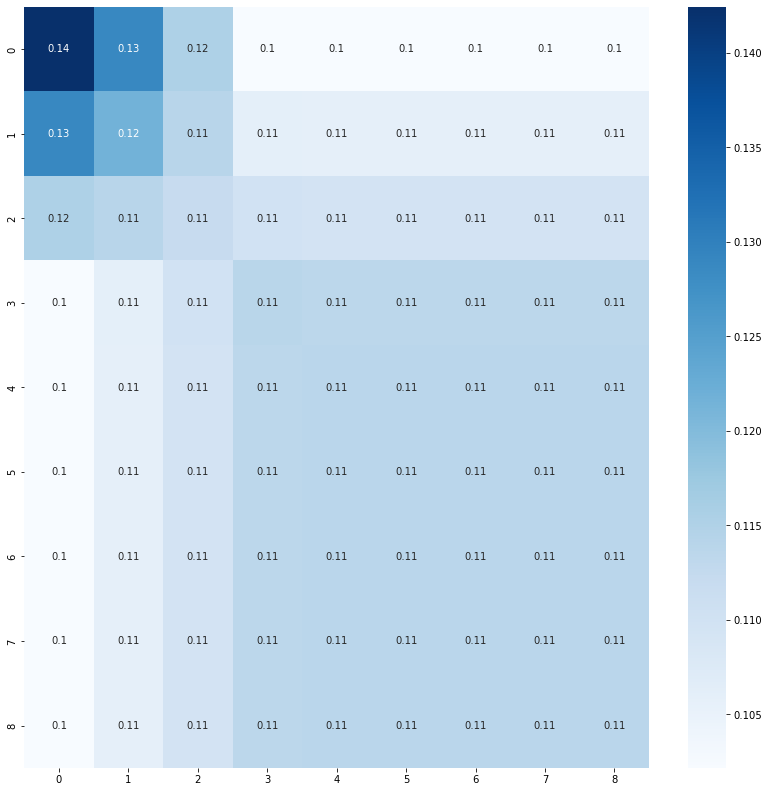
\includegraphics[width=0.4\textwidth]{naphthol_runs_old/vac_meth_overlap_old1}%
		\label{fig:naphtvacold1meth}%
	}\hfil
	\subfigure[Run 2]{%
		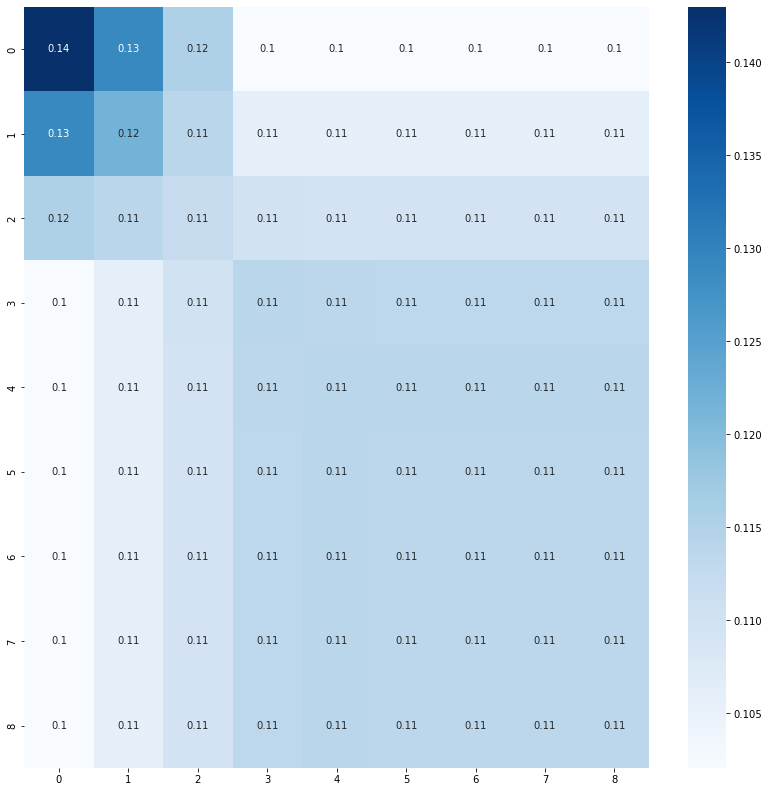
\includegraphics[width=0.4\textwidth]{naphthol_runs_old/vac_meth_overlap_old2}%
		\label{fig:naphtvacold2meth}%
	}
	
	\subfigure[Run 3]{%
		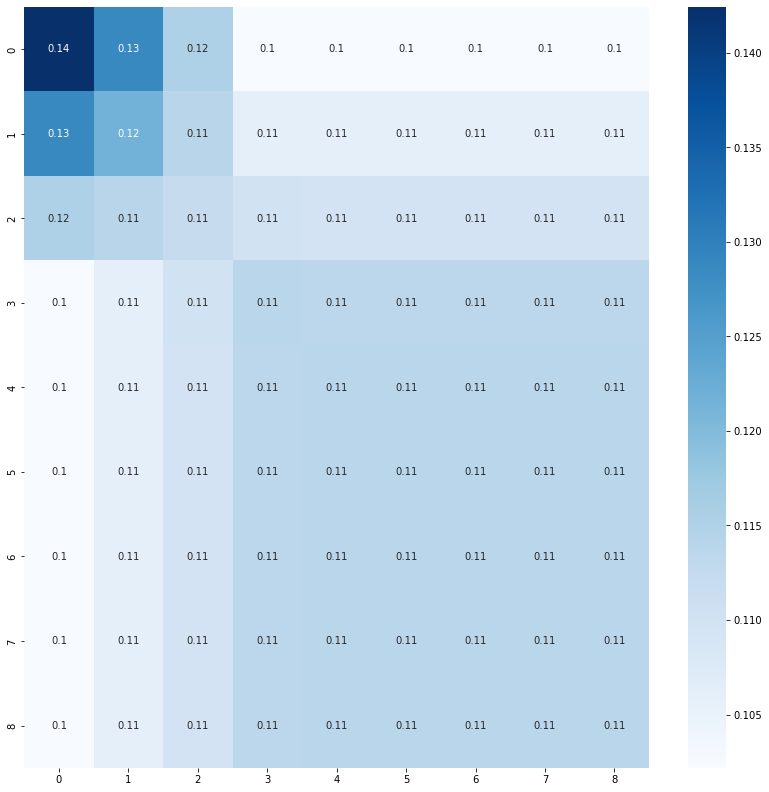
\includegraphics[width=0.4\textwidth]{naphthol_runs_old/vac_meth_overlap_old3}%
		\label{fig:naphtvacold3meth}%
	}\hfil
	\subfigure[Run 4]{%
		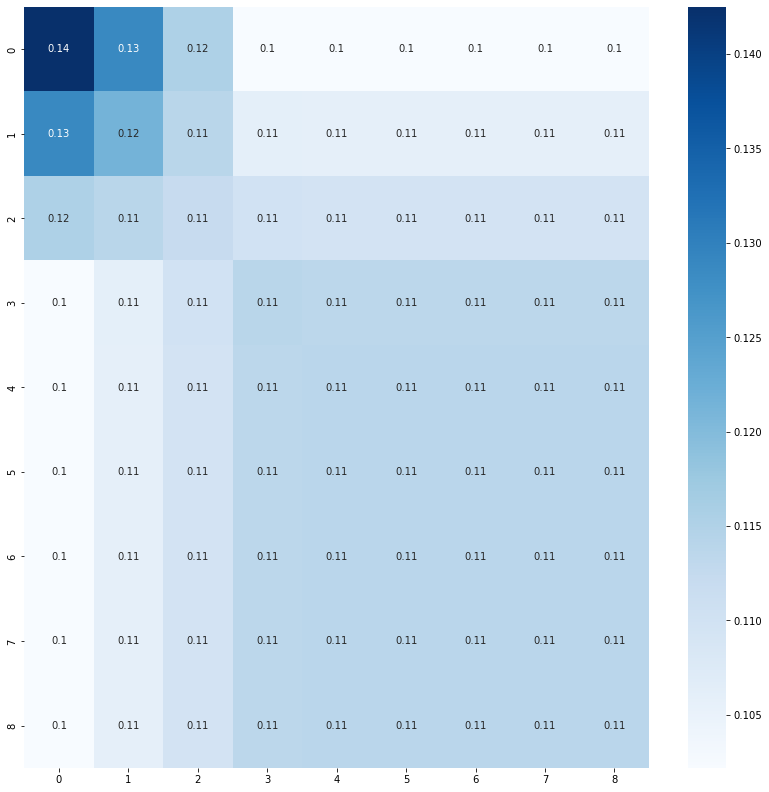
\includegraphics[width=0.4\textwidth]{naphthol_runs_old/vac_meth_overlap_old4}%
		\label{fig:naphtvacold4meth}%
	}
	
	\caption{Overlap plots for Methanol/Vacuum (from transformation 2-naphthol->methanol), old algorithm (As only one heavy atom is involved, the mutation algorithm obviously plays no role.)}
\end{figure}

\begin{figure}[htp]
	\centering
	\subfigure[Run 1]{%
		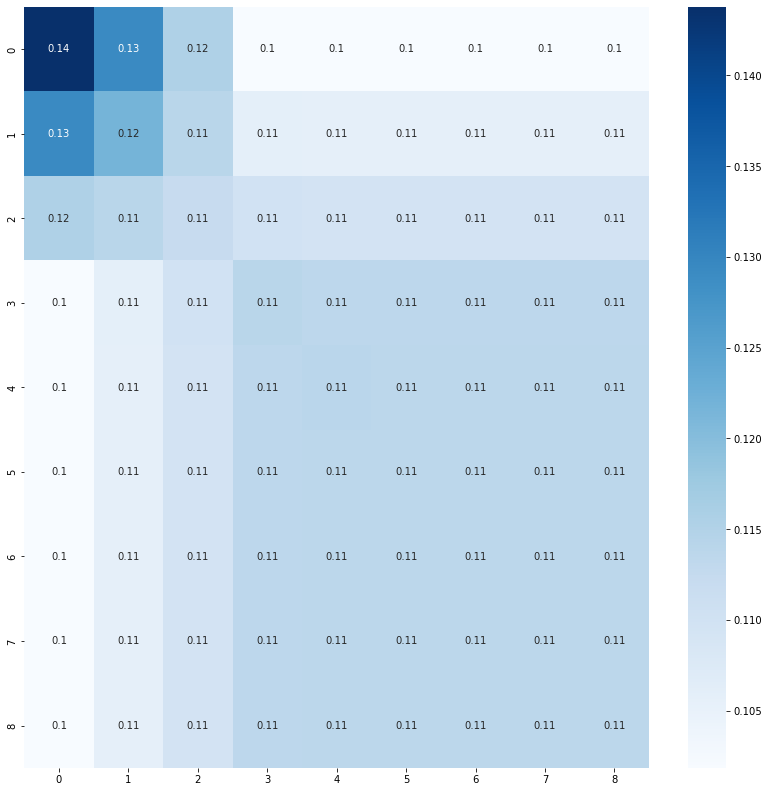
\includegraphics[width=0.4\textwidth]{naphthol_runs_new/vac_meth_overlap_new1}%
		\label{fig:naphtvacnew1meth}%
	}\hfil
	\subfigure[Run 2]{%
		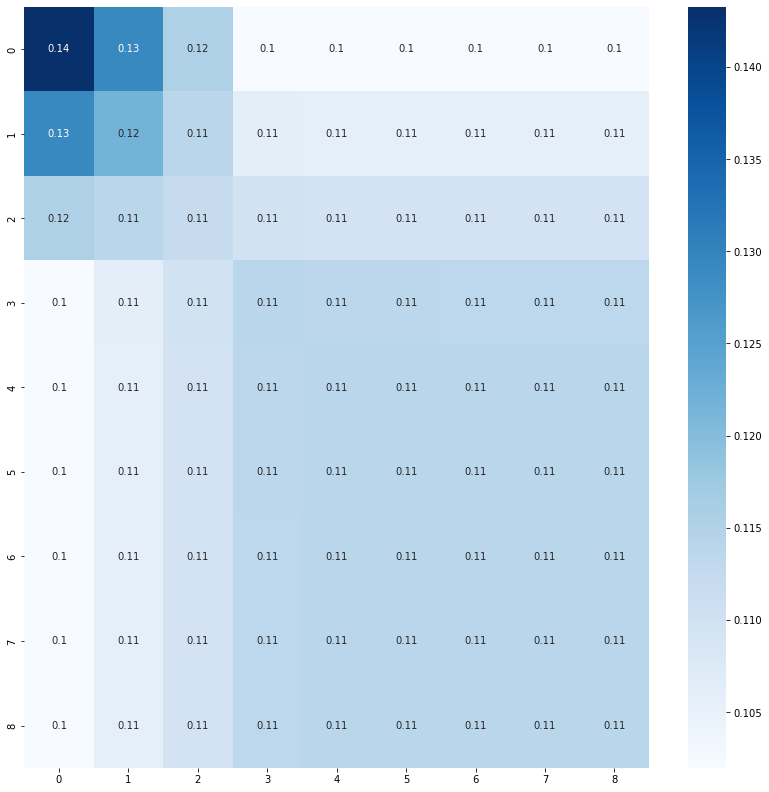
\includegraphics[width=0.4\textwidth]{naphthol_runs_new/vac_meth_overlap_new2}%
		\label{fig:naphtvacnew2meth}%
	}
	
	\subfigure[Run 3]{%
		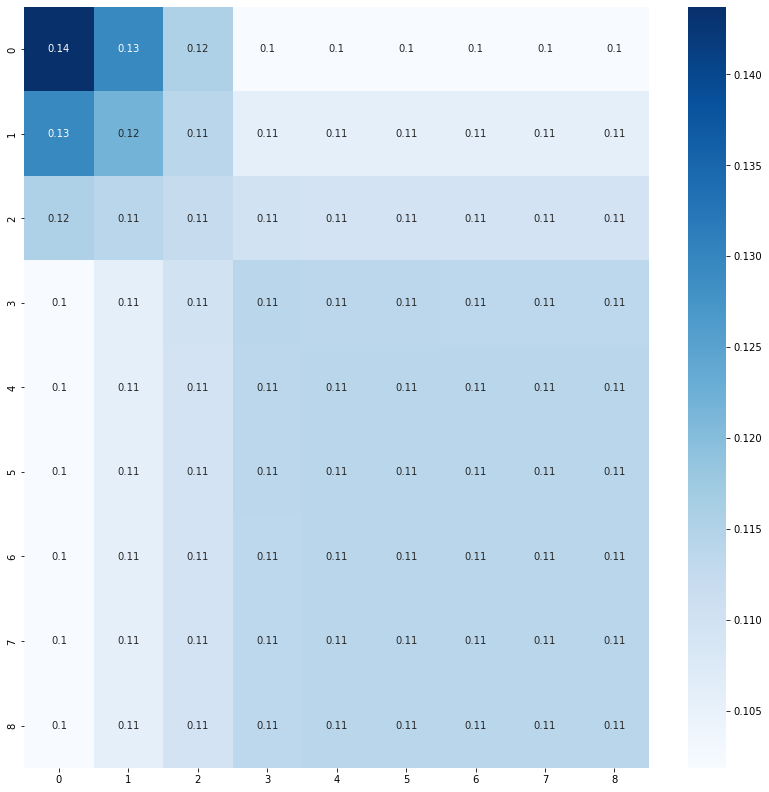
\includegraphics[width=0.4\textwidth]{naphthol_runs_new/vac_meth_overlap_new3}%
		\label{fig:naphtvacnew3meth}%
	}\hfil
	\subfigure[Run 4]{%
		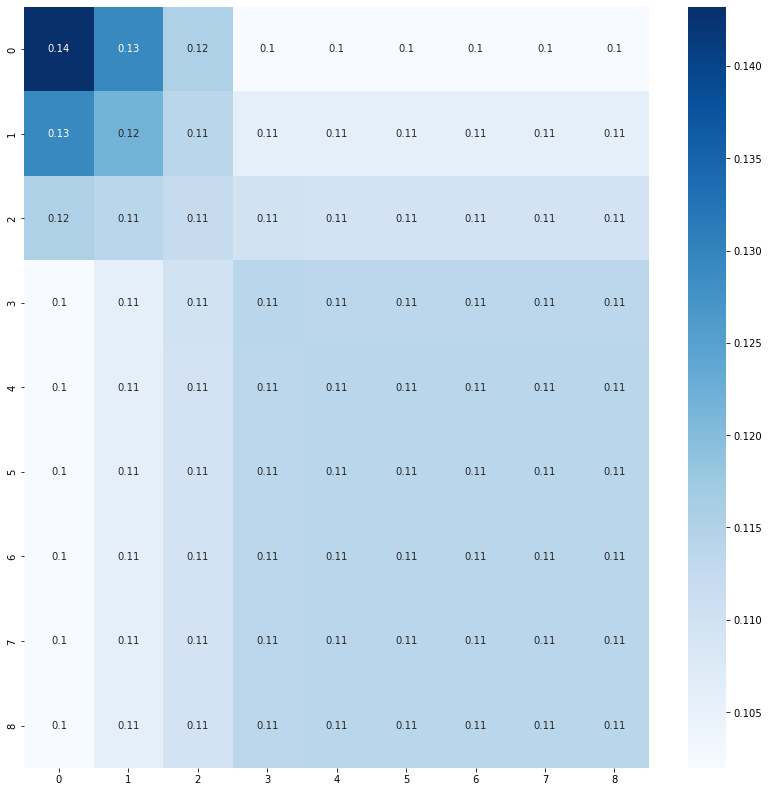
\includegraphics[width=0.4\textwidth]{naphthol_runs_new/vac_meth_overlap_new4}%
		\label{fig:naphtvacnew4meth}%
	}
	
	\caption{Overlap plots for Methanol/Vacuum (from transformation 2-naphthol->methanol), new algorithm (As only one heavy atom is involved, the mutation algorithm obviously plays no role.)}
\end{figure}





\begin{figure}[htp] 
	\centering
	\subfigure[Run 1]{%
		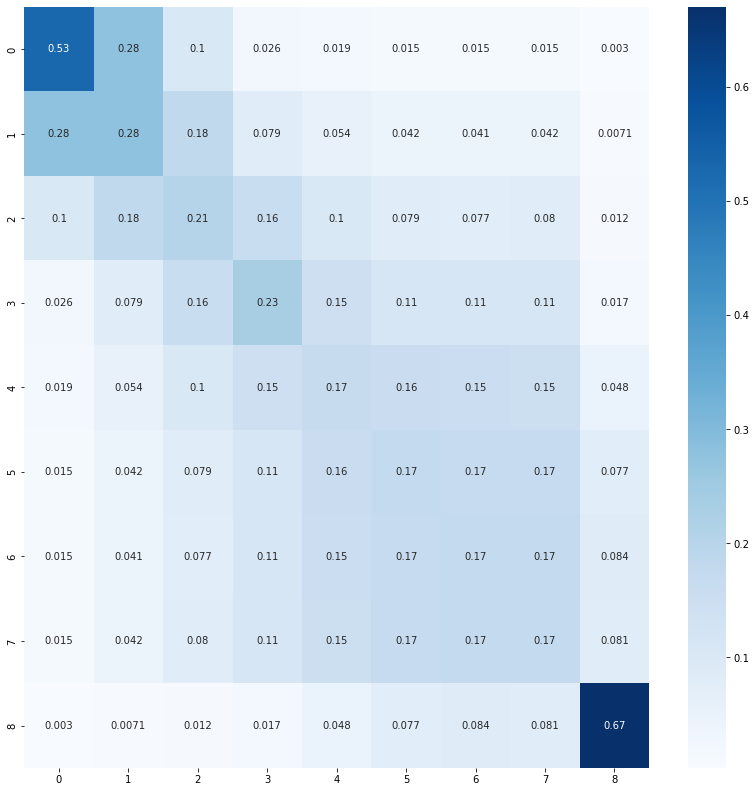
\includegraphics[width=0.4\textwidth]{naphthol_runs_old/waterbox_meth_overlap_old1}%
		\label{fig:naphtwatold1meth}%
	}\hfil
	\subfigure[Run 2]{%
		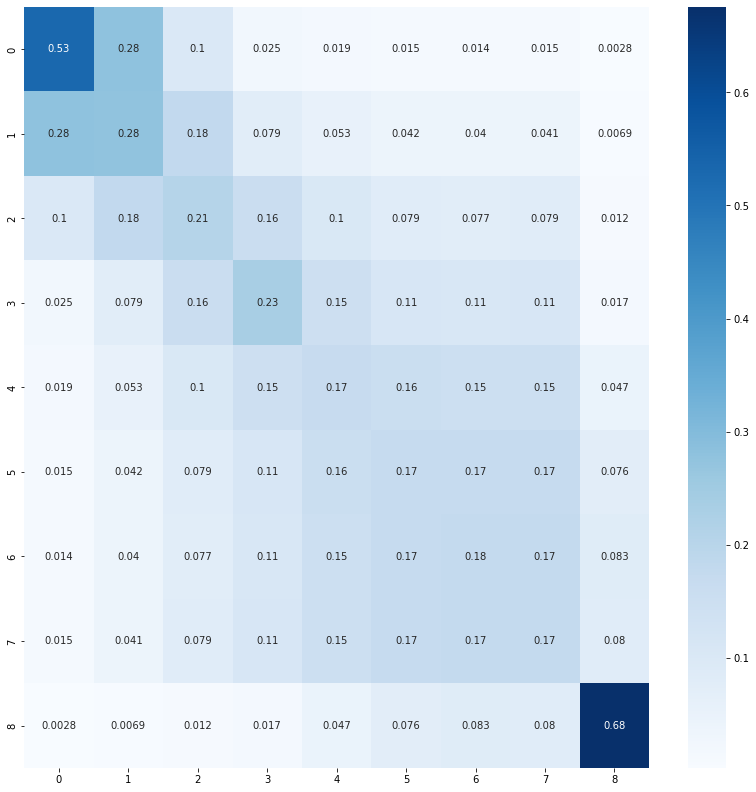
\includegraphics[width=0.4\textwidth]{naphthol_runs_old/waterbox_meth_overlap_old2}%
		\label{fig:naphtwatold2meth}%
	}
	
	\subfigure[Run 3]{%
		\includegraphics[width=0.4\textwidth]{naphthol_runs_old/waterbox_meth_overlap_old3}%
		\label{fig:naphtwatold3meth}%
	}\hfil
	\subfigure[Run 4]{%
		\includegraphics[width=0.4\textwidth]{naphthol_runs_old/waterbox_meth_overlap_old4}%
		\label{fig:naphtwatold4meth}%
	}
	
	\caption{Overlap plots for Methanol/Waterbox (from transformation 2-naphthol->methanol), old algorithm (As only one heavy atom is involved, the mutation algorithm obviously plays no role.)}
\end{figure}

\begin{figure}[htp] 
	\centering
	\subfigure[Run 1]{%
		\includegraphics[width=0.4\textwidth]{naphthol_runs_new/waterbox_meth_overlap_new1}%
		\label{fig:naphtwatnew1meth}%
	}\hfil
	\subfigure[Run 2]{%
		\includegraphics[width=0.4\textwidth]{naphthol_runs_new/waterbox_meth_overlap_new2}%
		\label{fig:naphtwatnew2meth}%
	}
	
	\subfigure[Run 3]{%
		\includegraphics[width=0.4\textwidth]{naphthol_runs_new/waterbox_meth_overlap_new3}%
		\label{fig:naphtwatnew3meth}%
	}\hfil
	\subfigure[Run 4]{%
		\includegraphics[width=0.4\textwidth]{naphthol_runs_new/waterbox_meth_overlap_new4}%
		\label{fig:naphtwatnew4meth}%
	}
	
	\caption{Overlap plots for Methanol/Waterbox (from transformation 2-naphthol->methanol), new algorithm (As only one heavy atom is involved, the mutation algorithm obviously plays no role.)}
\end{figure}


\begin{figure}[htp] 


	\includegraphics[width=0.9\textwidth]{old_new_runs_states}%
	

	\caption{comparison of the lambda states of the first simulation (possibly wrong results) and 4 runs of second simulation for toluene->methanol}
\end{figure}